\chapter{System Design}\label{ch:system-design}
The design baseline was produced in Part A (steps A1--A14) and lives in \code{docs/design/}, one folder per artefact kind. Diagrams follow their standard notation (UML 2.5; crow's foot for the ER diagram; Gane and Sarson for the DFD) and were reviewed against those notations in the A14 design review. Each figure below is followed by the reasoning behind it and the requirements it serves. Where the built system differs from a Part A diagram, the difference is stated and justified in Section~\ref{sec:design-evolution}.

\section{System Architecture}\label{sec:system-architecture}
Digital Mohalla is a \textbf{modular monolith}: one FastAPI service with strict internal layers, one PostgreSQL 16 database, and a React Native (Expo) client that runs on Android and the web. Figure~\ref{fig:layer-diagram} shows the layers.

\begin{figure}[htbp]
\centering
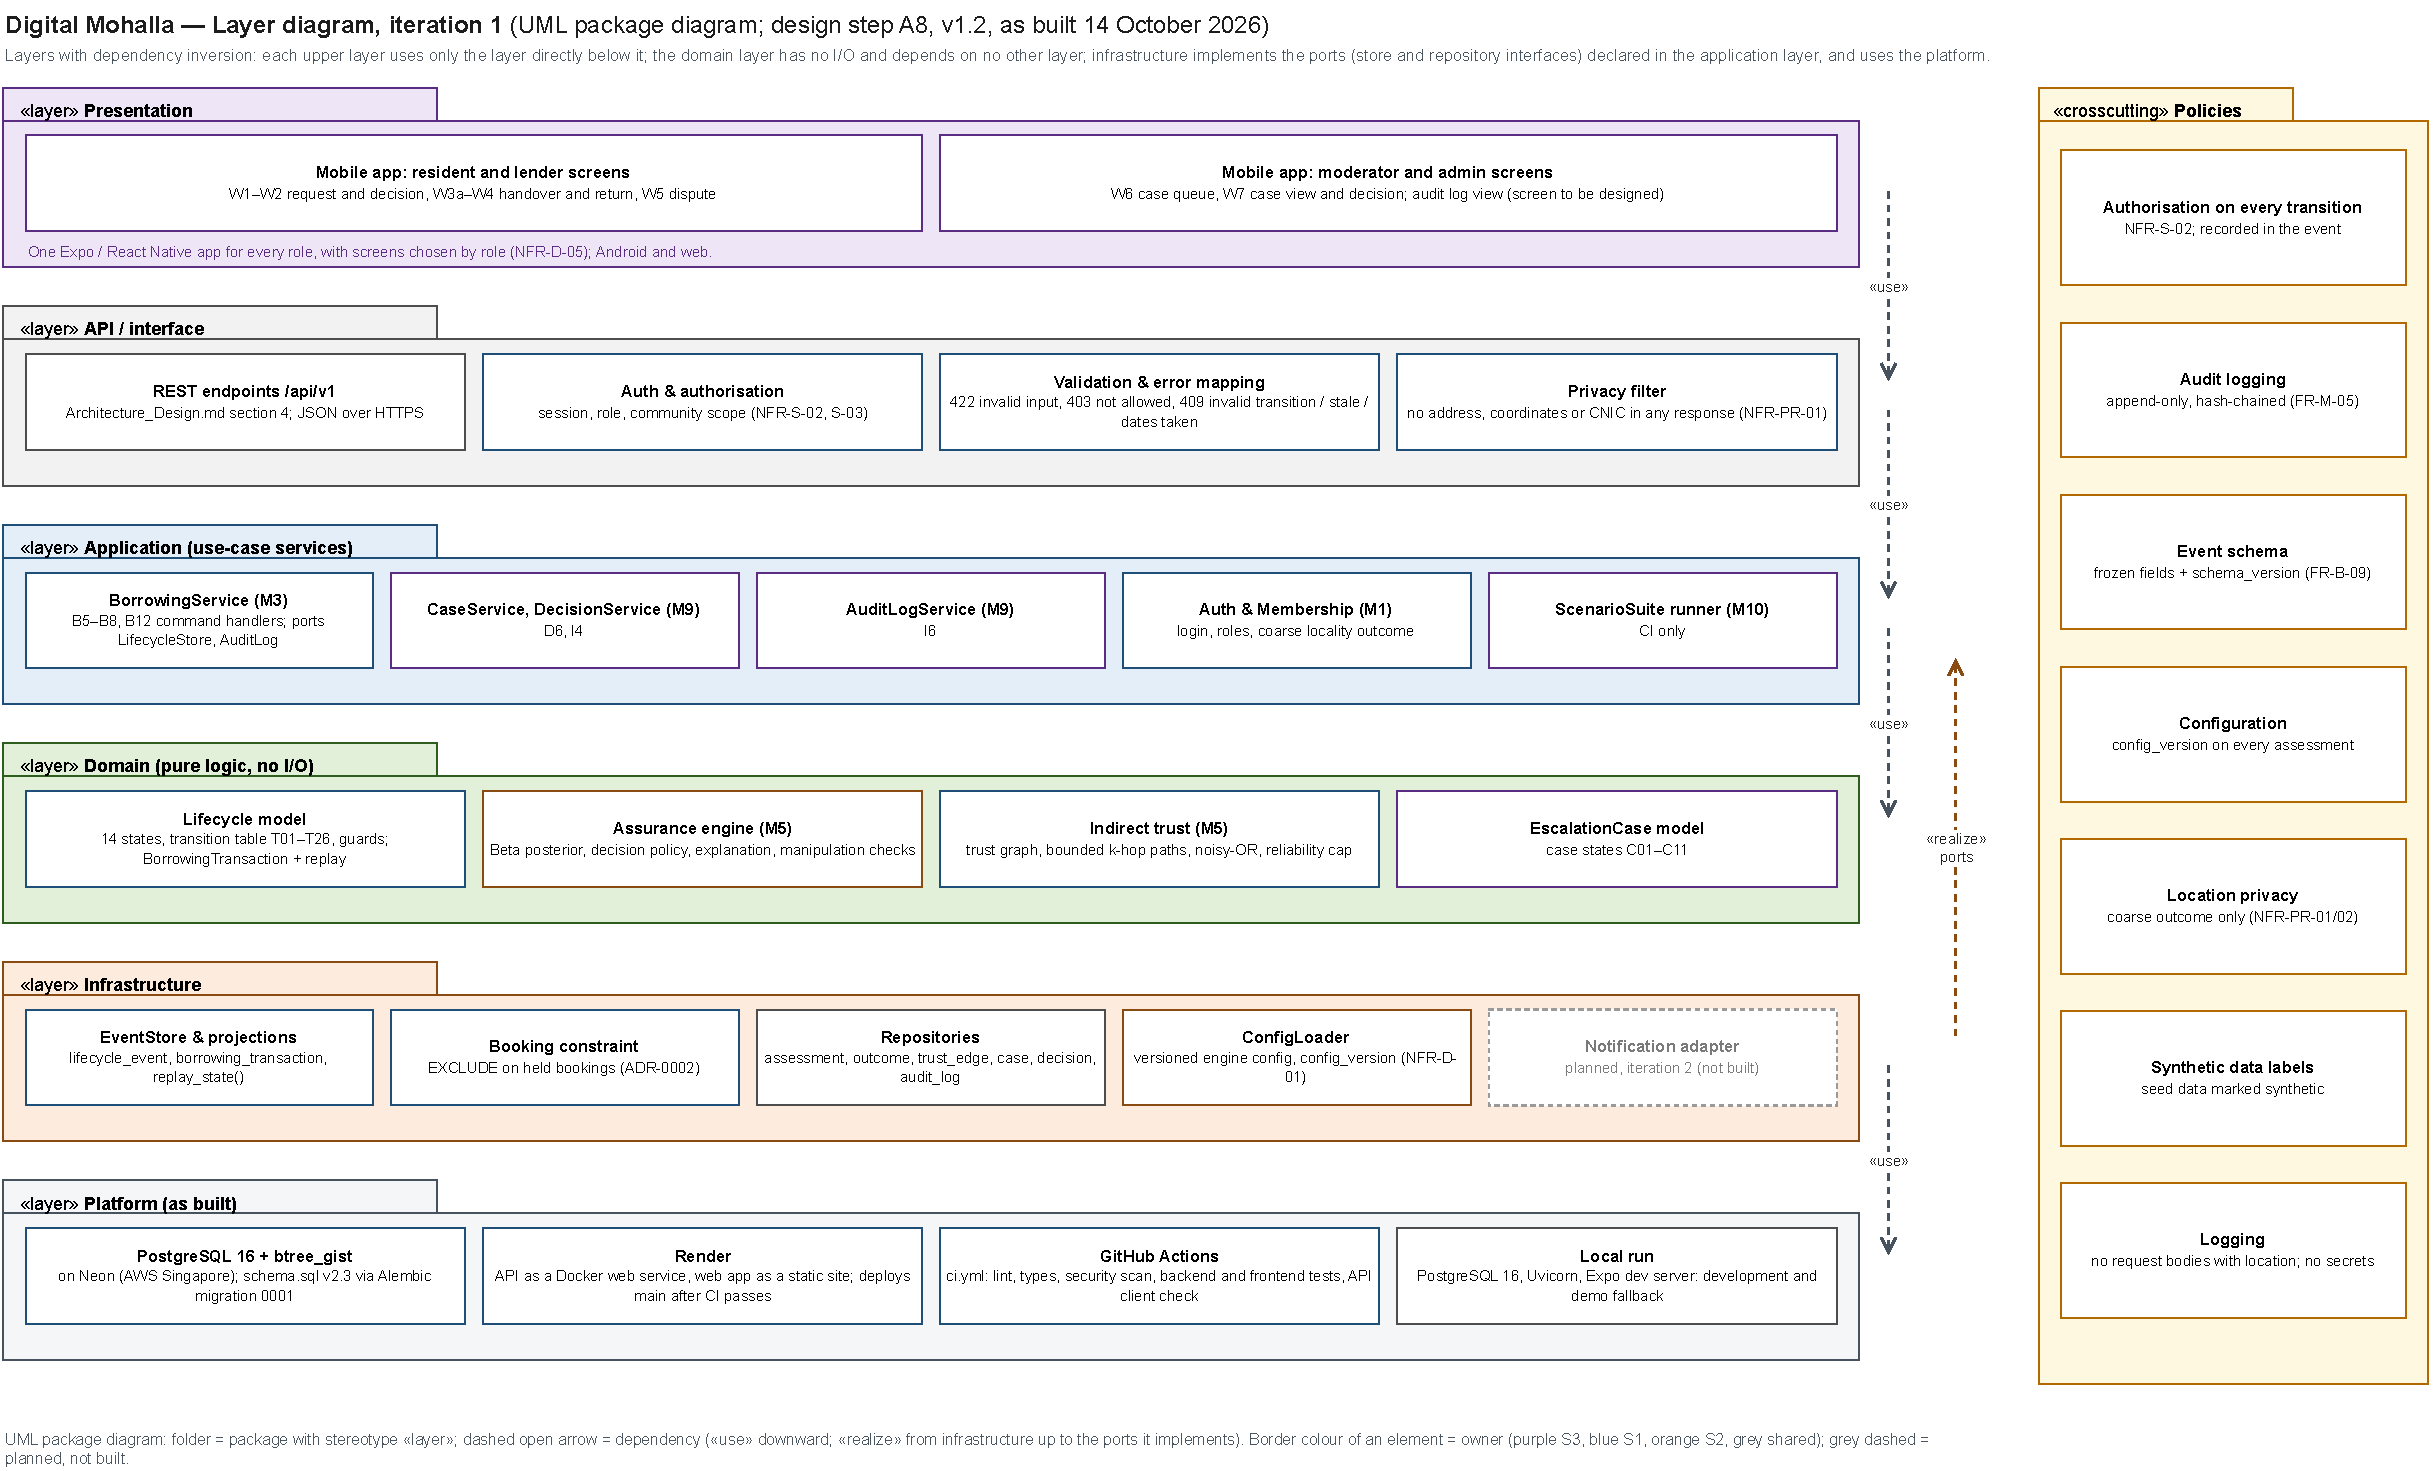
\includegraphics[width=\textwidth,height=0.80\textheight,keepaspectratio]{figures/diagrams/layer_diagram}
\caption{Layer diagram, Iteration 1 (UML package diagram, design step A8)}\label{fig:layer-diagram}
\drawionote{layer_diagram}{docs/design/03_architecture/layer_diagram.drawio}
\end{figure}

\textbf{Reasoning.} Each upper layer depends only on the one below it, and infrastructure depends upward on the ports it implements. The \textit{domain} layer (lifecycle model, assurance engine, moderation rules) is pure Python with no input/output, so the trust maths and the decision rules can be unit-tested without a database (477 unit tests run in seconds). Repositories are declared as interfaces in the application layer and implemented in infrastructure (dependency inversion), which is why the engine reaches the database only through the \code{EvidenceSource} interface. A monolith was chosen over services because three developers and one database do not need network boundaries, and a single transaction must cover the lifecycle transition, the booking and the event (ADR-0002). Cross-cutting policies (authorisation on every transition, the frozen event schema, \code{config_version} on every assessment, location privacy, synthetic labels) apply to every layer. \textit{Serves:} NFR-D-01, NFR-D-04, NFR-S-02, NFR-PR-01. \textit{Owner:} S1. The platform layer shows the deployed platform, Render and Neon (Section~\ref{sec:deployment}); the provisional AWS host of Part A is recorded in Section~\ref{sec:design-evolution}.

\section{Architectural Components}\label{sec:architectural-components}
Figure~\ref{fig:component-diagram} shows the ten modules, with the five worked on in Iteration 1 in detail.

\begin{figure}[p]
\centering
\begin{minipage}[c][0.92\textheight][c]{\textwidth}\centering
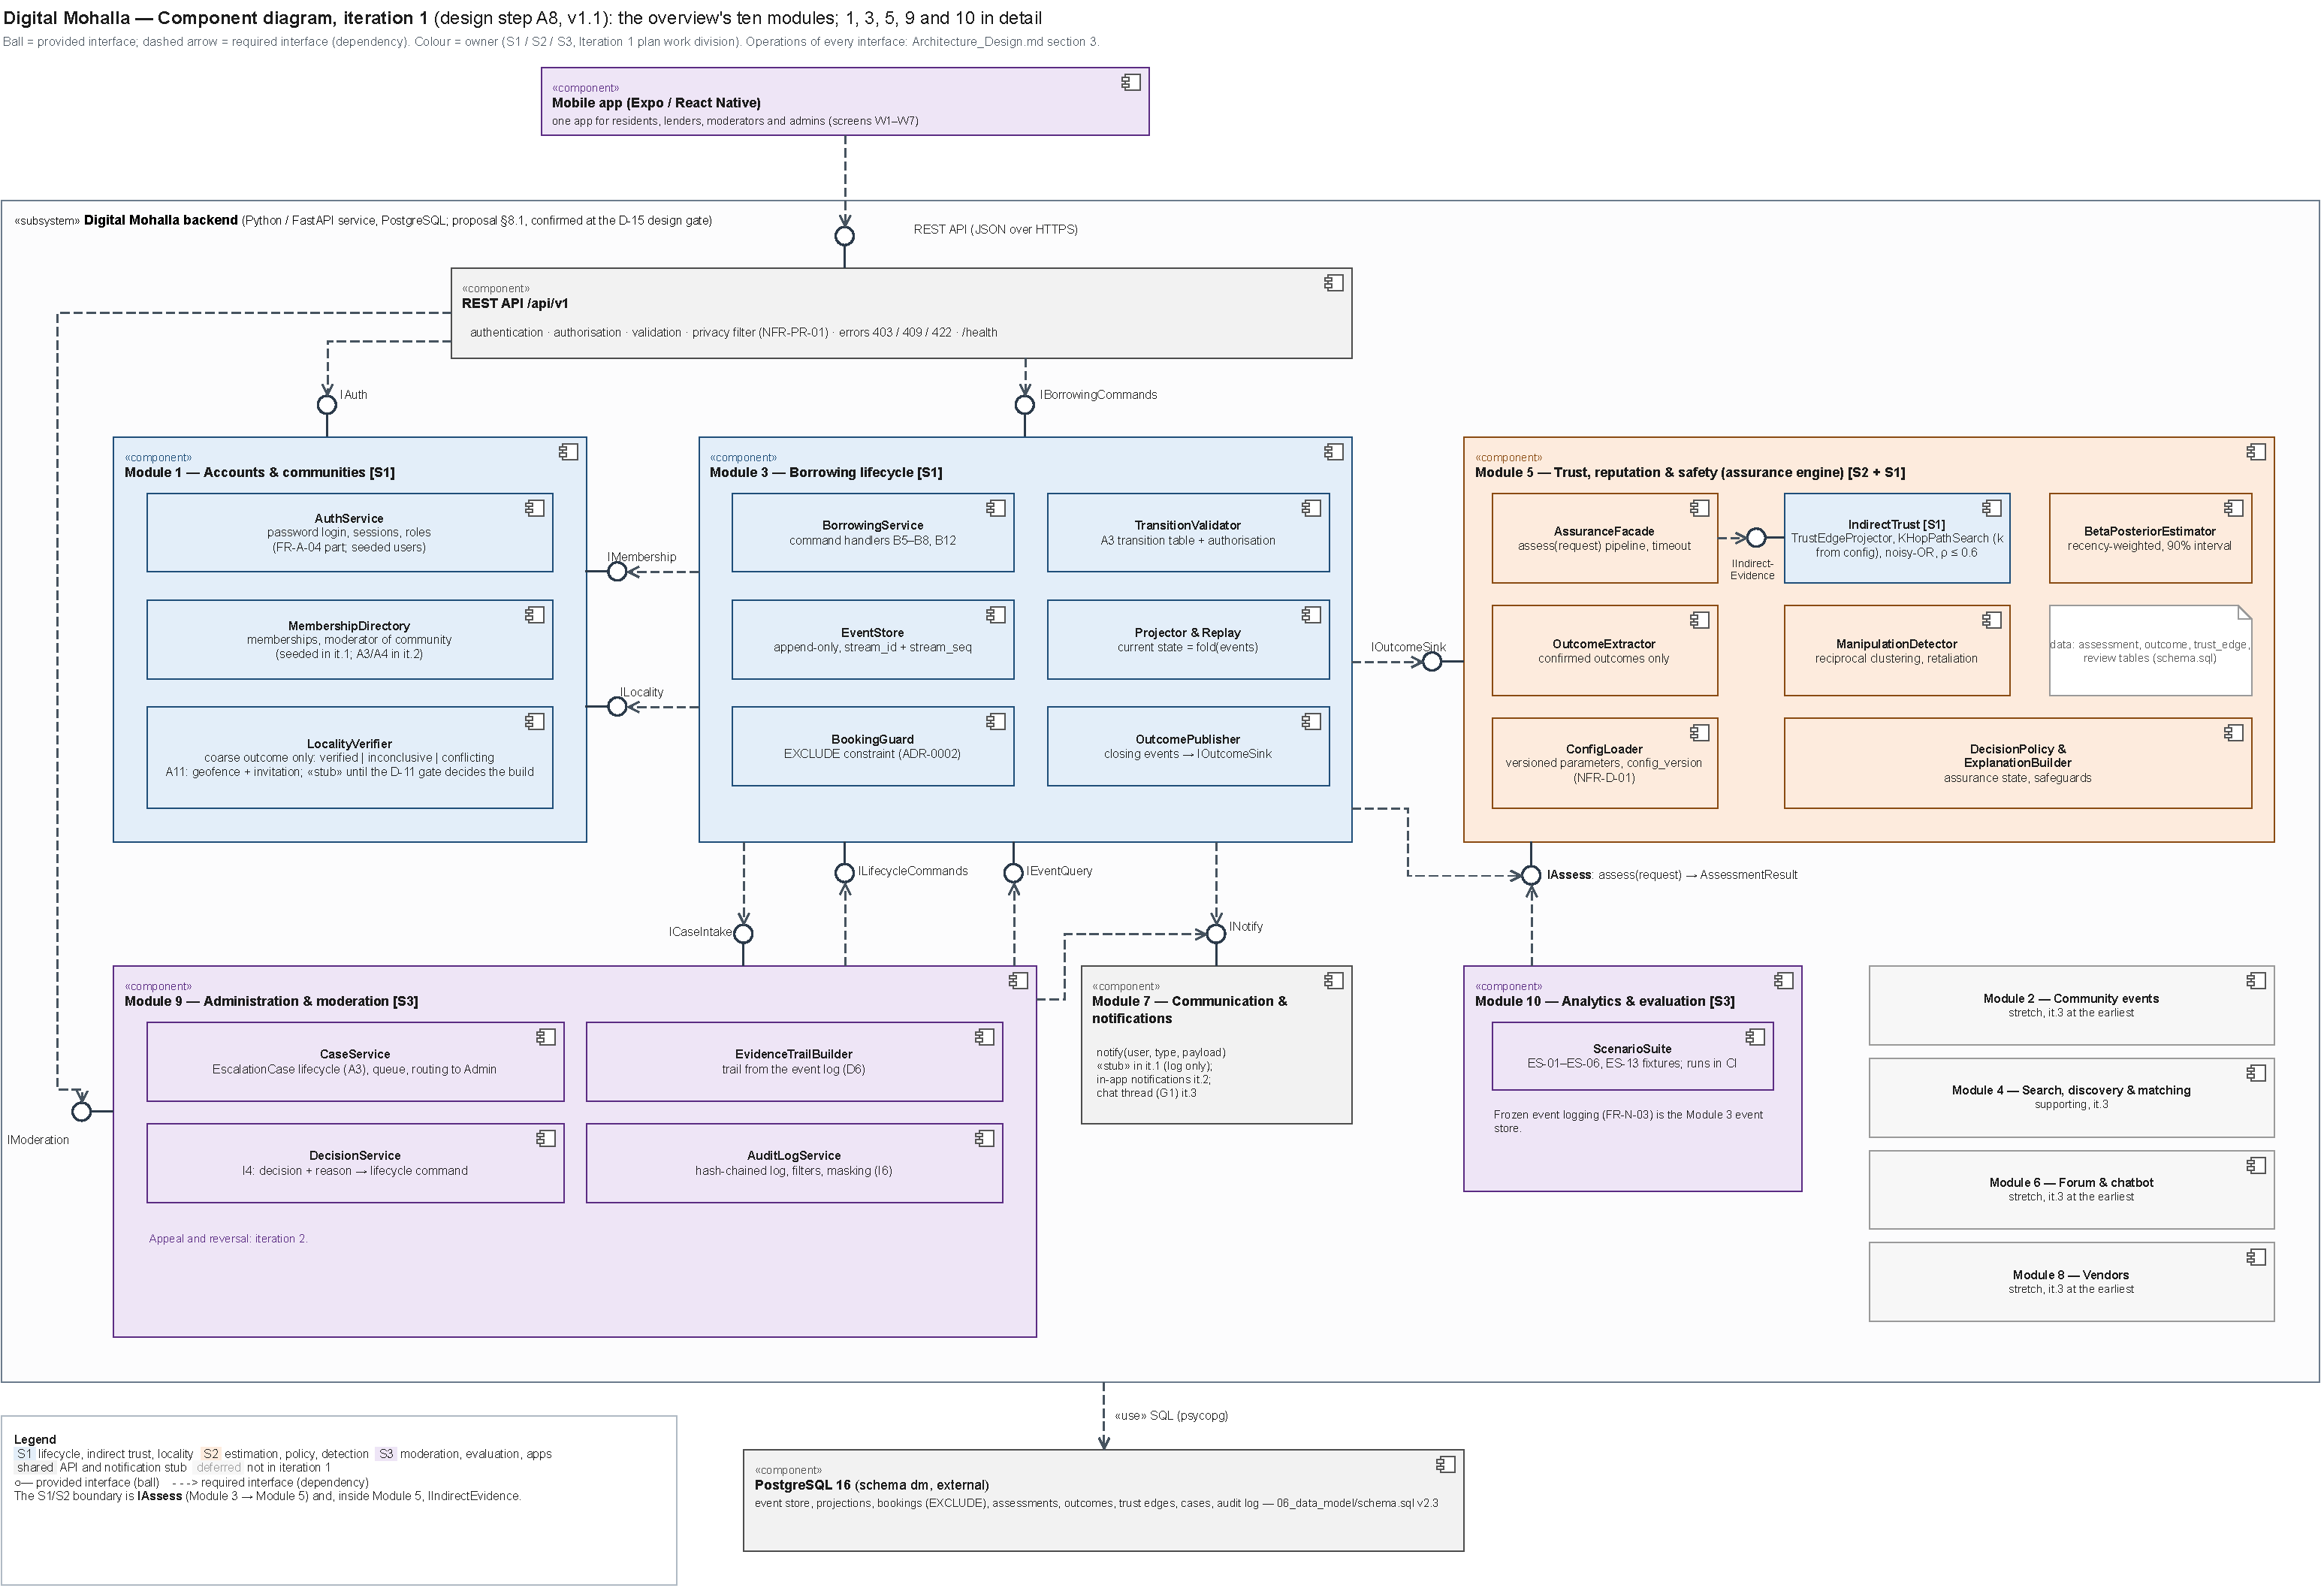
\includegraphics[width=\textwidth,height=0.80\textheight,keepaspectratio]{figures/diagrams/component_diagram}
\caption{Component diagram, Iteration 1 (UML 2.5, design step A8). Colour shows the owner (S1 blue, S2 orange, S3 purple)}\label{fig:component-diagram}
\drawionote{component_diagram}{docs/design/03_architecture/component_diagram.drawio}
\end{minipage}
\end{figure}

\textbf{Reasoning.} The diagram makes ownership and boundaries visible. Module 3 (lifecycle) and Module 5 (assurance) meet at exactly one provided interface, \code{IAssess.assess(request)}; inside Module 5 the S1/S2 boundary is the indirect-evidence interface. Module 3 calls the engine once per request, so a slow or failing engine affects one request and is turned into a hold (FR-T-07) instead of an error. Moderation (Module 9) changes the lifecycle only through lifecycle commands, so a moderator's decision passes the same transition checks as any other actor's. Modules 2, 4, 6 and 8 are drawn as deferred so the scope boundary is explicit. \textit{Serves:} FR-T-01, FR-T-07, FR-T-11, FR-B-08.

\textbf{From design components to code.} During implementation several design classes became plain functions or merged into one service, because Python modules and protocols gave the same boundaries with less code. Table~\ref{tab:design-components-mapped-implementation} maps every component in Figure~\ref{fig:component-diagram} to the code that realises it.

\begingroup\small
\begin{longtable}{@{}L{111pt}L{149pt}L{115pt}@{}}
\caption{Design components mapped to the implementation}\label{tab:design-components-mapped-implementation}\\
\toprule
Design element (A7/A8) & Implementation & Note \\
\midrule
\endfirsthead
\toprule
Design element (A7/A8) & Implementation & Note \\
\midrule
\endhead
\bottomrule
\endlastfoot
\code{IAssess} & \code{IAssess} protocol, \code{domain/lifecycle/ports.py} & As designed \\
\code{AssuranceFacade} & \code{AssuranceEngine.assess()}, \code{domain/assurance/engine.py} & Renamed \\
\code{BetaPosteriorEstimator} & \code{estimate()}, \code{credible_interval()}, \code{recency_weight()} in \code{estimation/posterior.py}; \code{similarity.py} & Functions instead of a class (pure) \\
\code{OutcomeExtractor}, \code{IOutcomeSink} & \code{estimation/outcomes.py} (rules) and \code{infra/db/outcomes.py} (writer), called from the close hook in \code{BorrowingService} & Interface replaced by a direct, idempotent call on loan close \\
\code{IndirectTrust}, \code{IIndirectEvidence}, \code{TrustEdgeProjector}, \code{KHopPathSearch} & \code{indirect/khop.py} (\code{find_paths}, \code{indirect_trust}), \code{indirect/edges.py}, \code{infra/db/trust_edges.py} & S1/S2 boundary kept as a module boundary \\
\code{ManipulationDetector}, \code{ReciprocalClustering}, \code{ReviewSimilarity}, \code{RetaliationCheck} & \code{detection/manipulation.py}: \code{partner_clustering}, \code{review_similarity}, retaliation set-aside, \code{combine} & S1 redefined as partner clustering (D18) \\
\code{DecisionPolicy}, \code{ExplanationBuilder} & \code{policy/decision.py} (\code{decide}, \code{RULES}), \code{policy/explanation.py} & As designed \\
\code{ConfigLoader} & \code{config/engine_config.py}, \code{config/engine.json} & As designed \\
\code{BorrowingService} & \code{BorrowingService}, \code{domain/lifecycle/service.py} & Also hosts dispute and moderation commands \\
\code{TransitionValidator} & \code{TransitionTable} (\code{transition_table.py}) and the database foreign key to \code{allowed_transition} & Checked twice \\
\code{EventStore}, \code{IEventQuery}, \code{Projector & Replay} & \code{LifecycleStore} protocol; \code{infra/eventstore/postgres.py}, \code{store.py}; \code{aggregate.py}; SQL \code{replay_state()} & As designed \\
\code{BookingGuard} & PostgreSQL exclusion constraint on \code{booking} & No Python class needed \\
\code{CaseService}, \code{DecisionService}, \code{ICaseIntake}, \code{IModeration} & \code{domain/moderation/decisions.py} (\code{plan}) and \code{BorrowingService.decide}, \code{moderation_queue}, \code{moderator_case} & Merged into the lifecycle service \\
\code{EvidenceTrailBuilder} & \code{BorrowingService.dispute_case}, \code{moderator_case} (trail read from \code{lifecycle_event}) & As designed \\
\code{AuditLogService} & \code{AuditLog} protocol; hash-chained \code{audit_log} table & Screen in Iteration 2 \\
\code{LocalityVerifier}, \code{ILocality} & \code{LifecycleStore.locality_outcome()} reading the stored result (\code{locality_outcome_for()}) & Stub; method in Iteration 2 \\
\code{INotify} & Not built & Iteration 2 \\
\code{AuthService}, \code{IAuth} & \code{domain/accounts/auth.py}, \code{api/deps.py} & Minimal login \\
\end{longtable}
\endgroup
\section{Interfaces and Dependencies}\label{sec:interfaces-dependencies}
\subsection{External interface: REST API}\label{sec:external-interface-rest-api}
The API is served under \code{/api/v1}, takes and returns JSON, and is described by an OpenAPI document from which the app's typed client is generated (a CI job fails if the two drift apart). Every request body refuses unknown fields, so a client cannot set the actor, the authorisation or the next state itself.

\begin{table}[!htbp]
\centering
\small
\caption{REST endpoints (Iteration 1)}\label{tab:rest-endpoints-iteration-1}
\begin{tabular}{@{}L{39pt}L{174pt}L{162pt}@{}}
\toprule
Method & Path & Purpose \\
\midrule
POST & \code{/auth/login} & Password login; returns a token \\
GET & \code{/items}, \code{/items/{id}} & Items visible to the member \\
POST & \code{/requests} & Create a borrowing request (UC-B5) \\
GET & \code{/requests}, \code{/requests/{id}}, \code{/lender/requests} & The member's requests; one request with its assessment; the lender's queue \\
POST & \code{/requests/{id}/accept}, \code{/decline}, \code{/cancel} & Lender decision; borrower cancellation (UC-B6) \\
POST & \code{/transactions/{id}/handover/checklist}, \code{/handover/confirm} & Handover (UC-B7) \\
POST & \code{/transactions/{id}/return}, \code{/return/confirm} & Return (UC-B8) \\
GET & \code{/transactions/{id}/events} & The event trail \\
POST, GET & \code{/transactions/{id}/dispute}, \code{/dispute/withdraw} & Raise, view and withdraw a dispute (UC-B12) \\
GET & \code{/moderation/cases}, \code{/moderation/cases/{id}} & Moderator queue and case view \\
POST & \code{/moderation/cases/{id}/decision} & Moderator decision with reason (UC-I4) \\
GET & \code{/health} & Liveness check for deployment \\
\bottomrule
\end{tabular}
\end{table}
Errors follow one mapping: 401 without a valid token, 403 for the wrong actor, 404 for data the member may not see, 409 for an invalid transition, a stale command or ``dates taken'', and 422 for invalid input.

\subsection{Internal interfaces}\label{sec:internal-interfaces}
\begin{itemize}
\item \code{IAssess.assess(AssessmentRequest) -> AssessmentResult}: the only way the lifecycle reaches the engine; called with a 2,000 ms timeout read from the configuration.
\item \code{LifecycleStore}: everything the lifecycle service needs from storage (create, append, view, assessments, cases, decisions, bookings), implemented on PostgreSQL.
\item \code{EvidenceSource}: what the engine reads (the borrower's outcomes, the trust graph, open and recent disputes, verification, reviews and complaints), so the engine itself has no database code.
\item \code{AuditLog}: records refused commands and privileged actions.
\end{itemize}

External dependencies are listed with versions and licences in Section~\ref{sec:external-components-dependencies}.

\section{Architecture Decisions and Rationale}\label{sec:architecture-decisions-rationale}
Eight ADRs record the decisions that shape the code. The hosting choice (Render and Neon instead of the provisional AWS host) is recorded as a design change (Table~\ref{tab:design-changes-since-proposal}); its ADR is pending. (\code{docs/design/03_architecture/DigitalMohalla_ADRs_Ver1.md}).

\begingroup
\begin{longtable}{@{}L{34pt}L{137pt}L{204pt}@{}}
\caption{Architecture decision records}\label{tab:architecture-decision-records}\\
\toprule
ADR & Decision & Rationale \\
\midrule
\endfirsthead
\toprule
ADR & Decision & Rationale \\
\midrule
\endhead
\bottomrule
\endlastfoot
0001 & Soft hold: pending requests mark dates as requested and block nothing & A lender should see all interest; blocking at request time would let one borrower lock an item with requests \\
0002 & The database enforces the no-overlap rule at acceptance (exclusion constraint on held bookings); transition, booking and event commit in one transaction & Replaces ``lower \code{stream_seq} wins'', which only orders events within one transaction and cannot arbitrate between two transactions \\
0003 & Exits from HELD\_FOR\_REVIEW depend on the hold reason (new event \code{hold_cleared}) & A cleared locality hold must still be assessed; a cleared manipulation hold already has an assessment; an engine-failure hold has nothing to attach safeguards to \\
0004 & Separate \code{dispute_resolved} and \code{dispute_withdrawn} events & A withdrawal restores the previous state; a resolution completes the loan and creates evidence; one event type could not mean both \\
0005 & Event-specific data goes in a \code{payload} field defined per event type & Keeps the frozen schema stable while each event carries its own data (dates, reasons, safeguards) \\
0006 & A trust edge's weight is the recency-weighted Beta posterior mean of the source's verified outcomes with the target (experimental) & One estimator for direct and indirect evidence; never a manual vouch \\
0007 & A manipulation hold needs corroboration (risk $\geq$60 and two signals $\geq$0.5); S4 active in Iteration 1 & ``$\geq$60 always holds'' contradicted the false-positive guard for real families; with one signal ES-04 could not be held at all \\
0008 & Community paths lift sparse direct evidence from INSUFFICIENT to REVIEW\_RECOMMENDED, never to SUFFICIENT & Without it the indirect evidence could never change a decision \\
\end{longtable}
\endgroup
Team decisions record the smaller choices: D1--D9 on 11 October (for example the \code{payload} field, no disputes from RETURNED, merging the Request table into the transaction) and D10--D20 on 13 October (Table~\ref{tab:team-decisions-d10-d20}).

\begingroup
\begin{longtable}{@{}L{26pt}L{136pt}L{213pt}@{}}
\caption{Team decisions D10--D20 (13 October 2026)}\label{tab:team-decisions-d10-d20}\\
\toprule
\# & Topic & Decision \\
\midrule
\endfirsthead
\toprule
\# & Topic & Decision \\
\midrule
\endhead
\bottomrule
\endlastfoot
D10 & Trust-edge weight & ADR-0006 accepted as experimental \\
D11 & Outcome mapping & Borrower: on-time return, condition agreed, dispute-free; lender: condition agreed, dispute-free; a party found at fault fails the relevant metrics \\
D12 & SUFFICIENT\_EVIDENCE thresholds & Mean $\geq 0.75$, lower 90\% bound $\geq 0.60$, $n_{\mathrm{eff}} \geq 3$, $\rho_{\mathrm{sup}} = 0.3$: initial hypotheses \\
D13 & ES-05 expected result & R8, SUFFICIENT\_EVIDENCE with safeguards: the retaliatory review is detected and set aside \\
D14 & ES-13 expected result & R9, REVIEW\_RECOMMENDED; without the community paths, R6\_SPARSE \\
D15 & Device scope & Android only for device testing; iOS not targeted \\
D16 & Test plan use & Tools added only when a test first needs them \\
D17 & Similarity of a past loan & $0.4\times$ value-band closeness $+\,0.4\times$ same category $+\,0.2\times$ duration closeness, floor 0.5 (S2) \\
D18 & Meaning of S1 & Partner clustering instead of pairwise reciprocity (confirmed by S2, 14 October) \\
D19 & Effect of a retaliation flag & The review is set aside from S1 and S4 and explained; reviews never enter the trust estimate (confirmed by S2, 14 October) \\
D20 & Photo uploads & Deferred to Iteration 2 (confirmed by S1 and S2, 14 October) \\
\end{longtable}
\endgroup
\section{Design Evolution}\label{sec:design-evolution}
\begingroup
\begin{longtable}{@{}L{111pt}L{111pt}L{153pt}@{}}
\caption{Design changes since the proposal}\label{tab:design-changes-since-proposal}\\
\toprule
Proposal / earlier design & Now & Why \\
\midrule
\endfirsthead
\toprule
Proposal / earlier design & Now & Why \\
\midrule
\endhead
\bottomrule
\endlastfoot
Nine technical components M1--M9 across a broad platform & Ten modules; the assurance engine is the core, stretch modules deferred & Panel point 3; the handbook's scope test needs a technical core per student \\
Trust shared by all three students & S1 indirect trust, S2 estimation/policy/detection, S3 moderation/evaluation & Each member owns a removable technical part \\
FAISS search, learning-to-rank, LightGBM & Search in Iteration 3; detection is rule-based and interpretable & No labelled data for a trained detector; every signal must be explainable to a moderator \\
Four reputation tiers & Four assurance states that describe evidence, not people & A tier labels a person; a state describes this loan's evidence \\
``Lower \code{stream_seq} wins'' for double booking & Database exclusion constraint (ADR-0002) & Correct across transactions and atomic \\
``RESUME'' to end a dispute & \code{dispute_resolved} / \code{dispute_withdrawn} (ADR-0004) & Different outcomes need different events \\
Separate Request table & Merged into \code{borrowing_transaction} (D7) & One stream per loan from request to close \\
Any risk $\geq$60 holds & Two corroborating signals needed (ADR-0007) & Protects real families (C3 guard) \\
Indirect evidence with no effect on the decision & R6\_SPARSE / R9 (ADR-0008) & Makes ES-13 decidable \\
Pairwise reciprocity signal & Partner clustering (D18) & Two-sided reviews are reciprocal by nature; the pairwise rule flagged 6 of 8 ordinary members \\
GPS sent with every request & Request carries no location; membership-time result is read (D13) & Privacy boundary moves to joining a community \\
One AWS host with Docker Compose (A13, provisional) & Render (API container and static web app) with Neon PostgreSQL & No server administration; deploys from \code{main} after CI \\
Design interfaces such as \code{IOutcomeSink}, \code{IIndirectEvidence} & Four protocols (\code{IAssess}, \code{LifecycleStore}, \code{EvidenceSource}, \code{AuditLog}) & Same boundaries, less code (Table~\ref{tab:design-components-mapped-implementation}) \\
\end{longtable}
\endgroup
\section{Domain Model}\label{sec:domain-model}
\textbf{Reasoning.} The central class is the \textit{BorrowingTransaction}, whose state is derived from its \textit{LifecycleEvents}; an \textit{Assessment} is attached to a transaction, not to a user, because an assurance state describes the evidence for one loan. \textit{Outcome} is separate from \textit{Review}: trust is computed only from verified outcomes, and reviews feed only the manipulation signals (D19), which is why a retaliatory review cannot lower anyone's trust. \textit{Booking}, \textit{ConditionReport} and \textit{LocalityResult} were kept as classes (integration decision of 11 October) because each is realised by a table and guarded by a database rule. \textit{Serves:} FR-B-09, FR-T-01, FR-T-03, FR-T-09.

\begin{figure}[p]
\centering
\begin{minipage}[c][0.92\textheight][c]{\textwidth}\centering
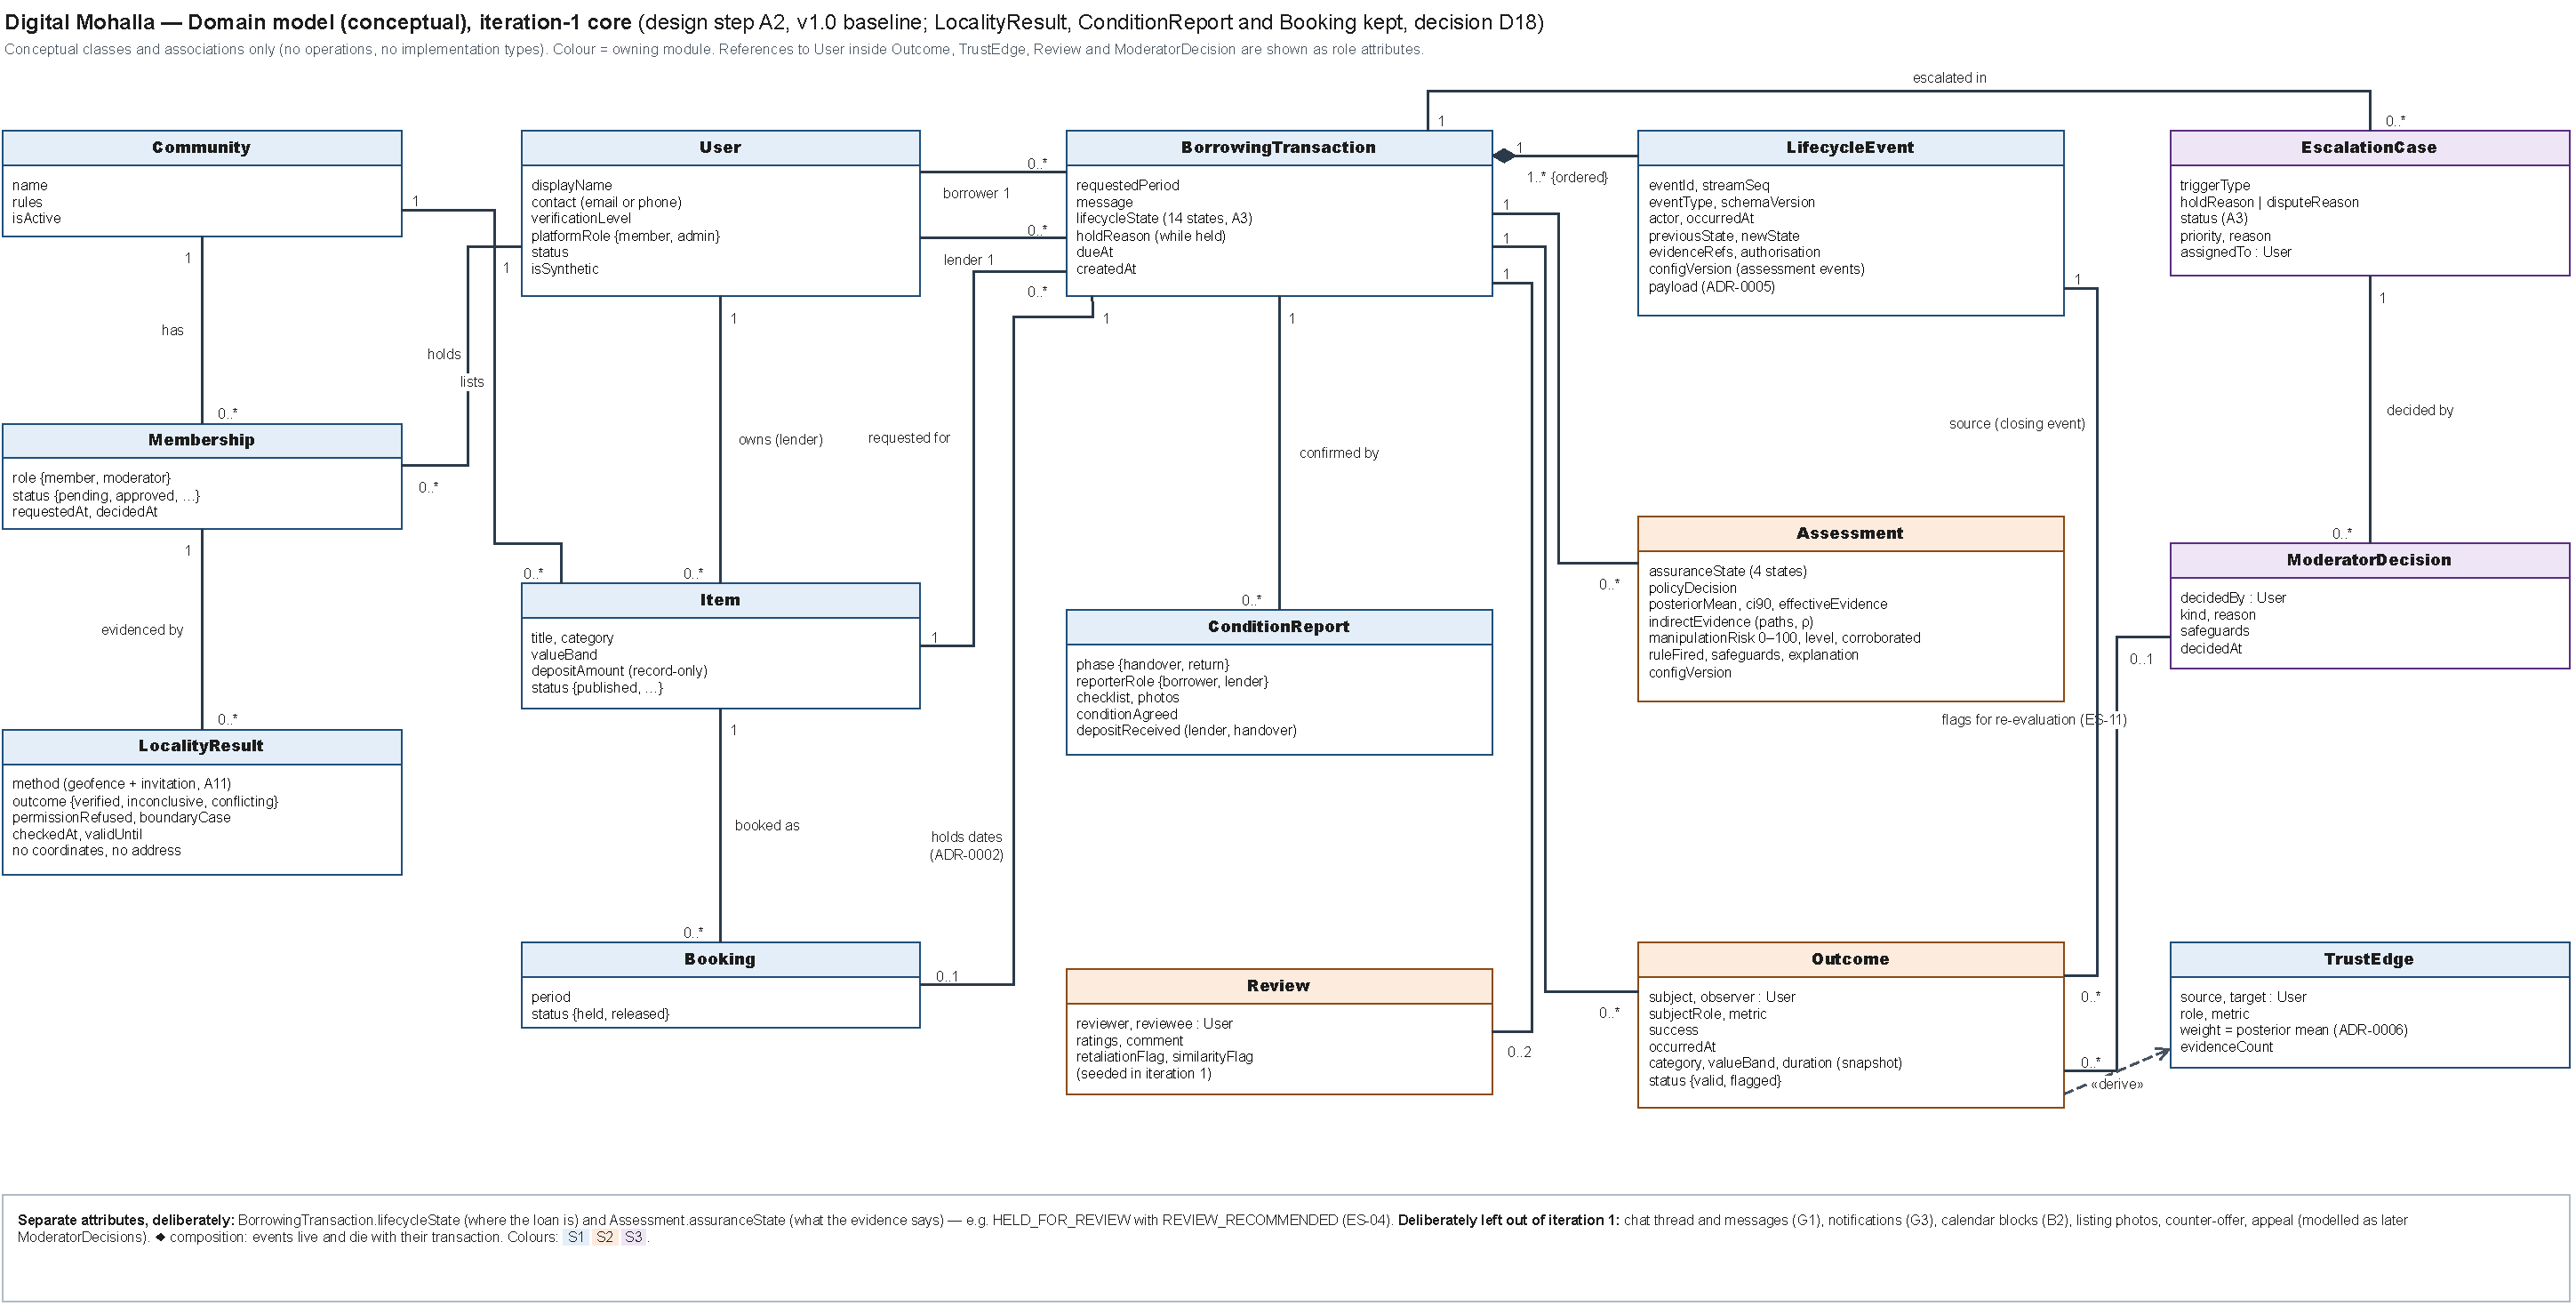
\includegraphics[width=\textwidth,height=0.80\textheight,keepaspectratio]{figures/diagrams/domain_model}
\caption{Domain model v1.0 (UML class diagram without operations, design step A2)}\label{fig:domain-model}
\drawionote{domain_model}{docs/design/05_class_model/domain_model.drawio}
\end{minipage}
\end{figure}

\section{Data Design}\label{sec:data-design}
\textbf{Reasoning.} The schema (\code{schema.sql} v2.3, applied by Alembic migration \code{0001}) enforces the rules that must never depend on application code:

\begin{itemize}
\item \textbf{Event store.} \code{lifecycle_event} is append-only (a trigger refuses UPDATE and DELETE) and hash-chained (\code{prev_hash}, \code{row_hash}); \code{verify_event_chain()} detects any altered row. \code{(stream_id, stream_seq)} is unique.
\item \textbf{Valid transitions.} \code{(previous_state, event_type, new_state)} is a composite foreign key to \code{allowed_transition}, so an invalid transition cannot be stored even if the Python check had a bug. The trigger \code{event_validate} checks the actor and sequence; \code{event_apply} updates the projection.
\item \textbf{Bookings.} \code{EXCLUDE (item_id WITH =, period WITH &&) WHERE held}, using \code{btree_gist}.
\item \textbf{Assessments.} Every row stores \code{config_version} (NOT NULL); \code{assessment_rule_ck} refuses a row whose rule, state, decision and hold reason disagree with the decision table.
\item \textbf{Privacy.} No column stores coordinates, an address or a CNIC; a test scans the catalogue for such columns.
\end{itemize}

\begin{figure}[p]
\centering
\begin{minipage}[c][0.92\textheight][c]{\textwidth}\centering
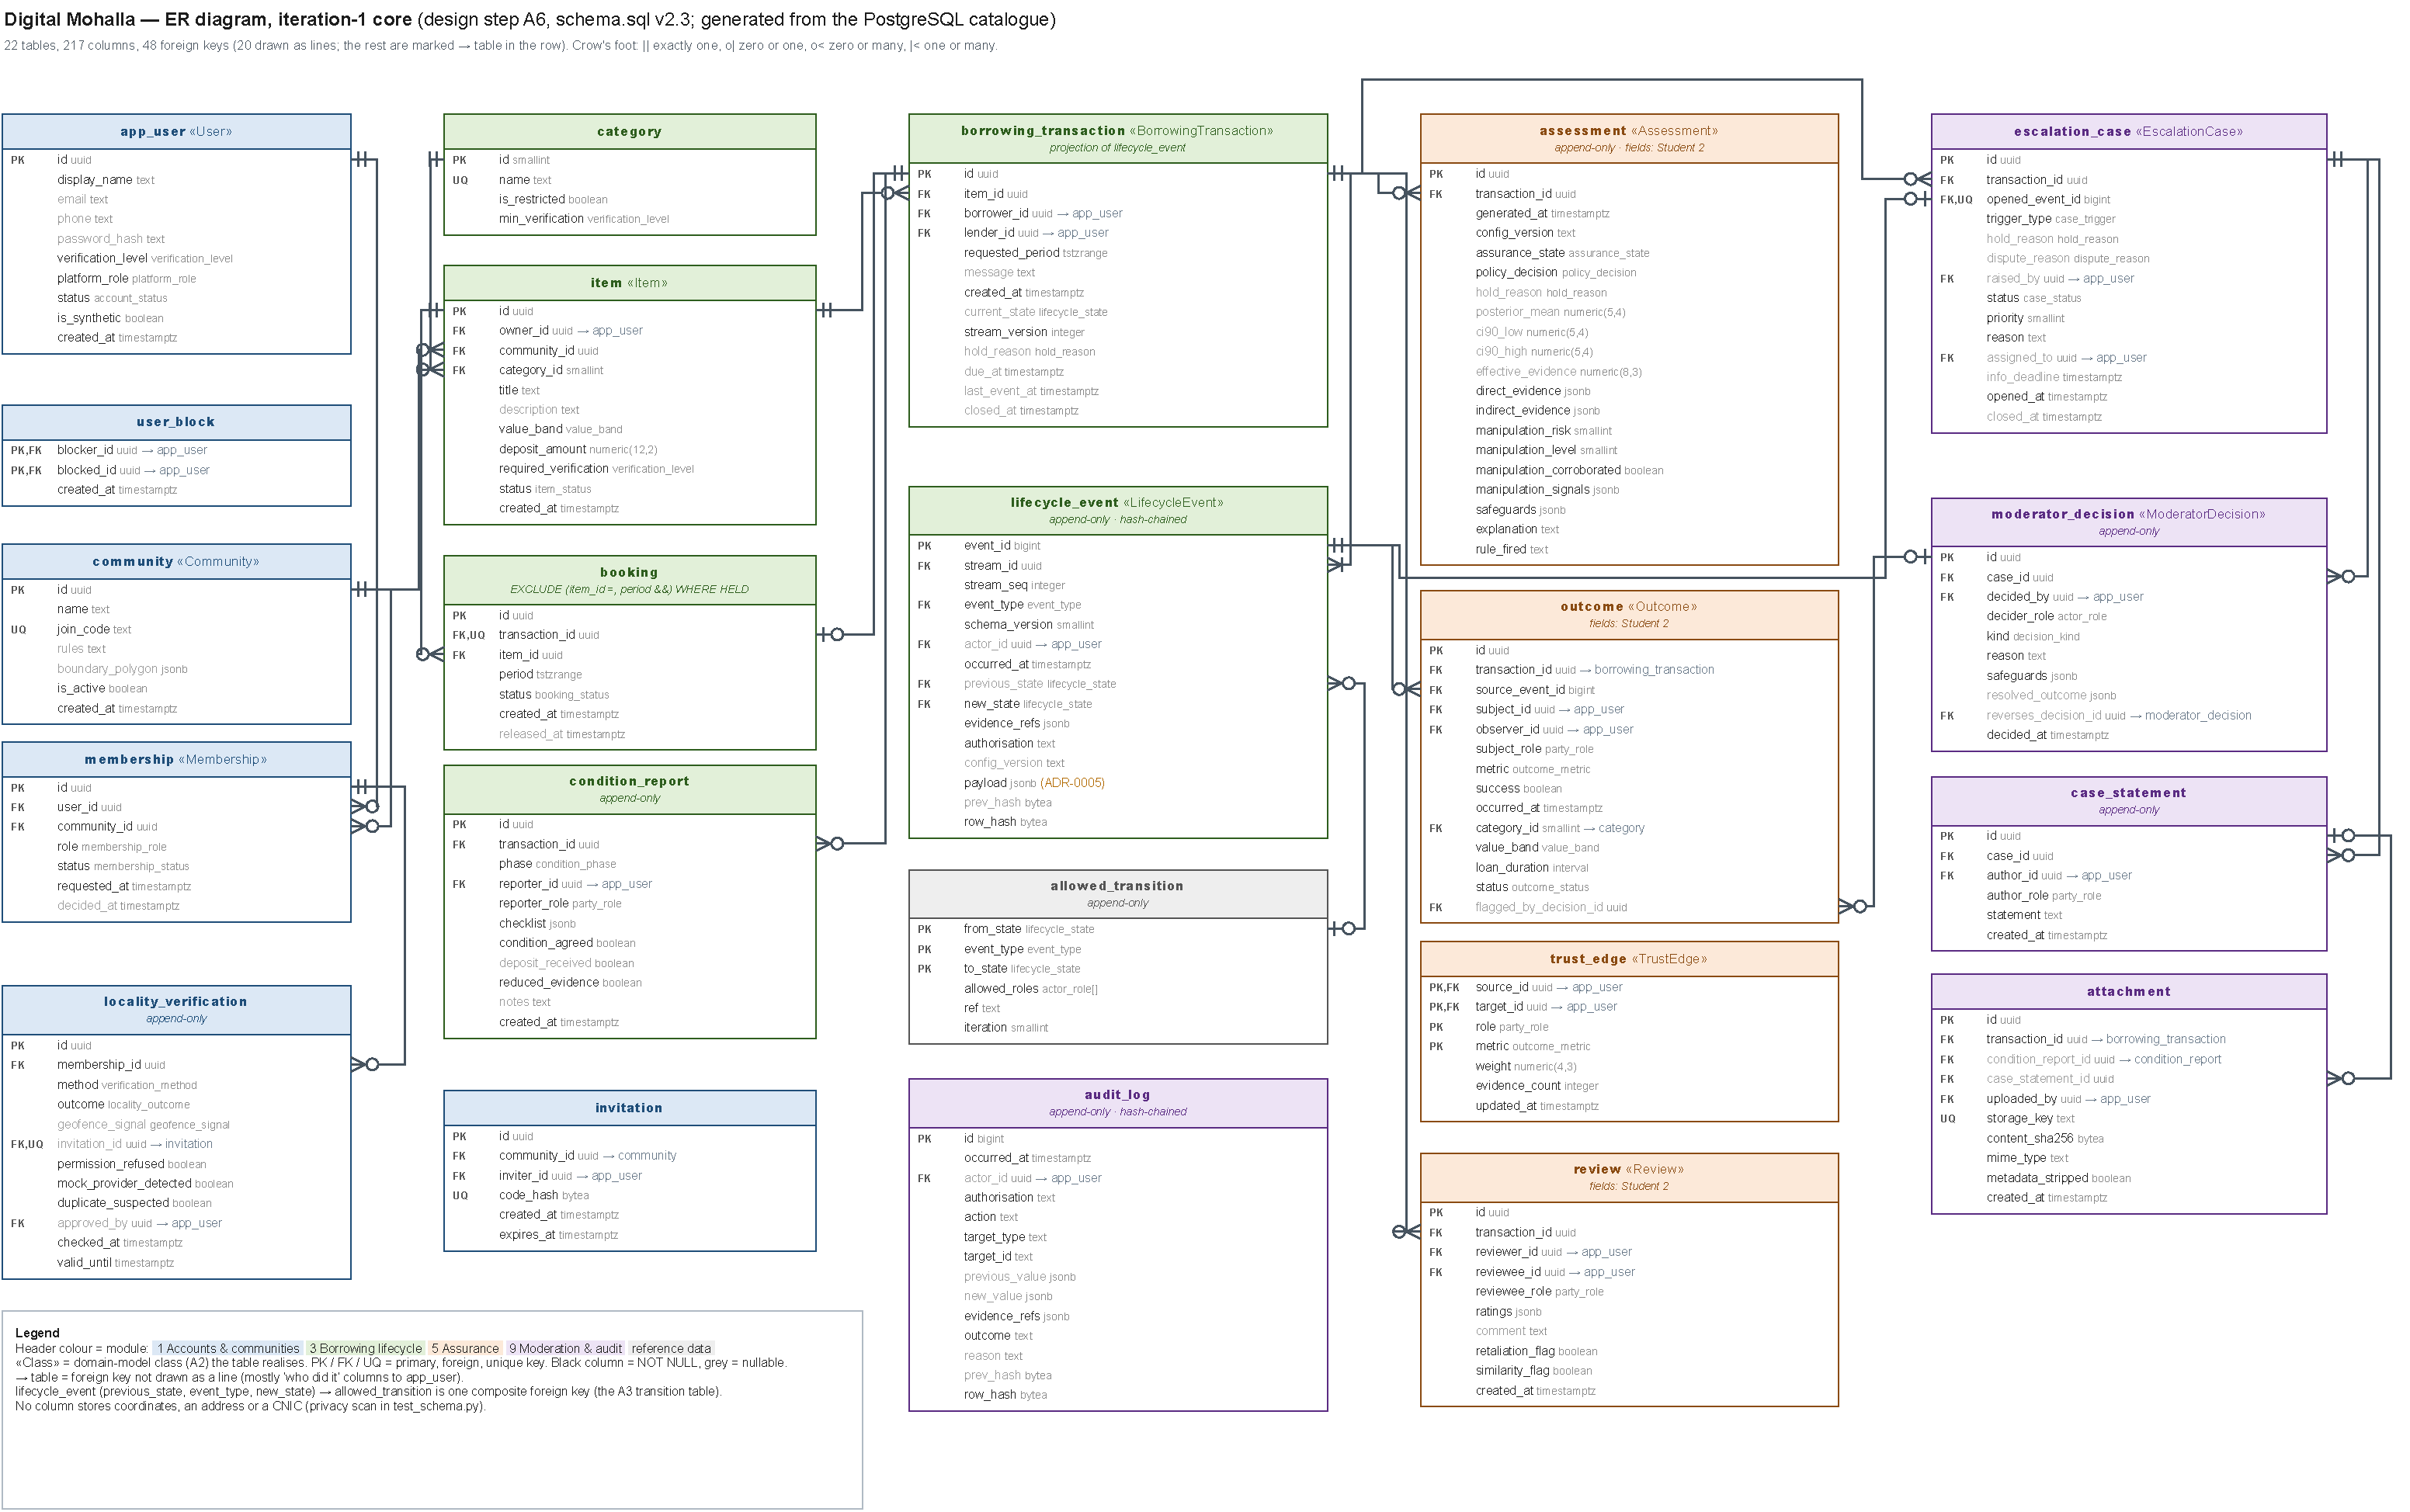
\includegraphics[width=\textwidth,height=0.80\textheight,keepaspectratio]{figures/diagrams/er_diagram}
\caption{ER diagram, schema v2.3 (crow's foot, design step A6): 22 tables, 217 columns, 48 foreign keys}\label{fig:er-diagram}
\drawionote{er_diagram}{docs/design/06_data_model/er_diagram.drawio}
\end{minipage}
\end{figure}

The current state is a projection (\code{borrowing_transaction.current_state}) that \code{replay_state()} can rebuild from the events alone. \textit{Serves:} FR-B-05, FR-B-08, FR-B-09, FR-M-05, NFR-D-01, NFR-PR-01. \textit{Owner:} S1 (lifecycle tables), S2 (assessment, outcome, trust edge, review fields).

\section{Process / Behavior Design}\label{sec:process-behavior-design}
\subsection{Borrowing lifecycle}\label{sec:borrowing-lifecycle}
\textbf{Reasoning.} Fourteen states in two composites: PENDING (dates only requested) and IN\_PROGRESS (booking held). Transitions that apply to every substate of a composite are drawn once on its border, and DISPUTED returns through a shallow-history state to the state stored in \code{dispute_opened}. HELD\_FOR\_REVIEW is never an automatic rejection: each hold reason has its own exits (ADR-0003). With the 21 event types this gives 294 state--event pairs, of which 31 are valid; the 31 valid pairs yield 34 leaf transitions because some events have guarded alternatives (for example \code{hold_cleared} returns to LOCALITY\_CHECKED or ASSESSED depending on the hold reason). Transitions marked ``it.2'' (expiry, no-show, extensions) are part of the table but are triggered by the Iteration 2 scheduler. \textit{Serves:} FR-B-08, FR-B-16, FR-B-17, FR-T-07.

\begin{figure}[p]
\centering
\begin{minipage}[c][0.92\textheight][c]{\textwidth}\centering
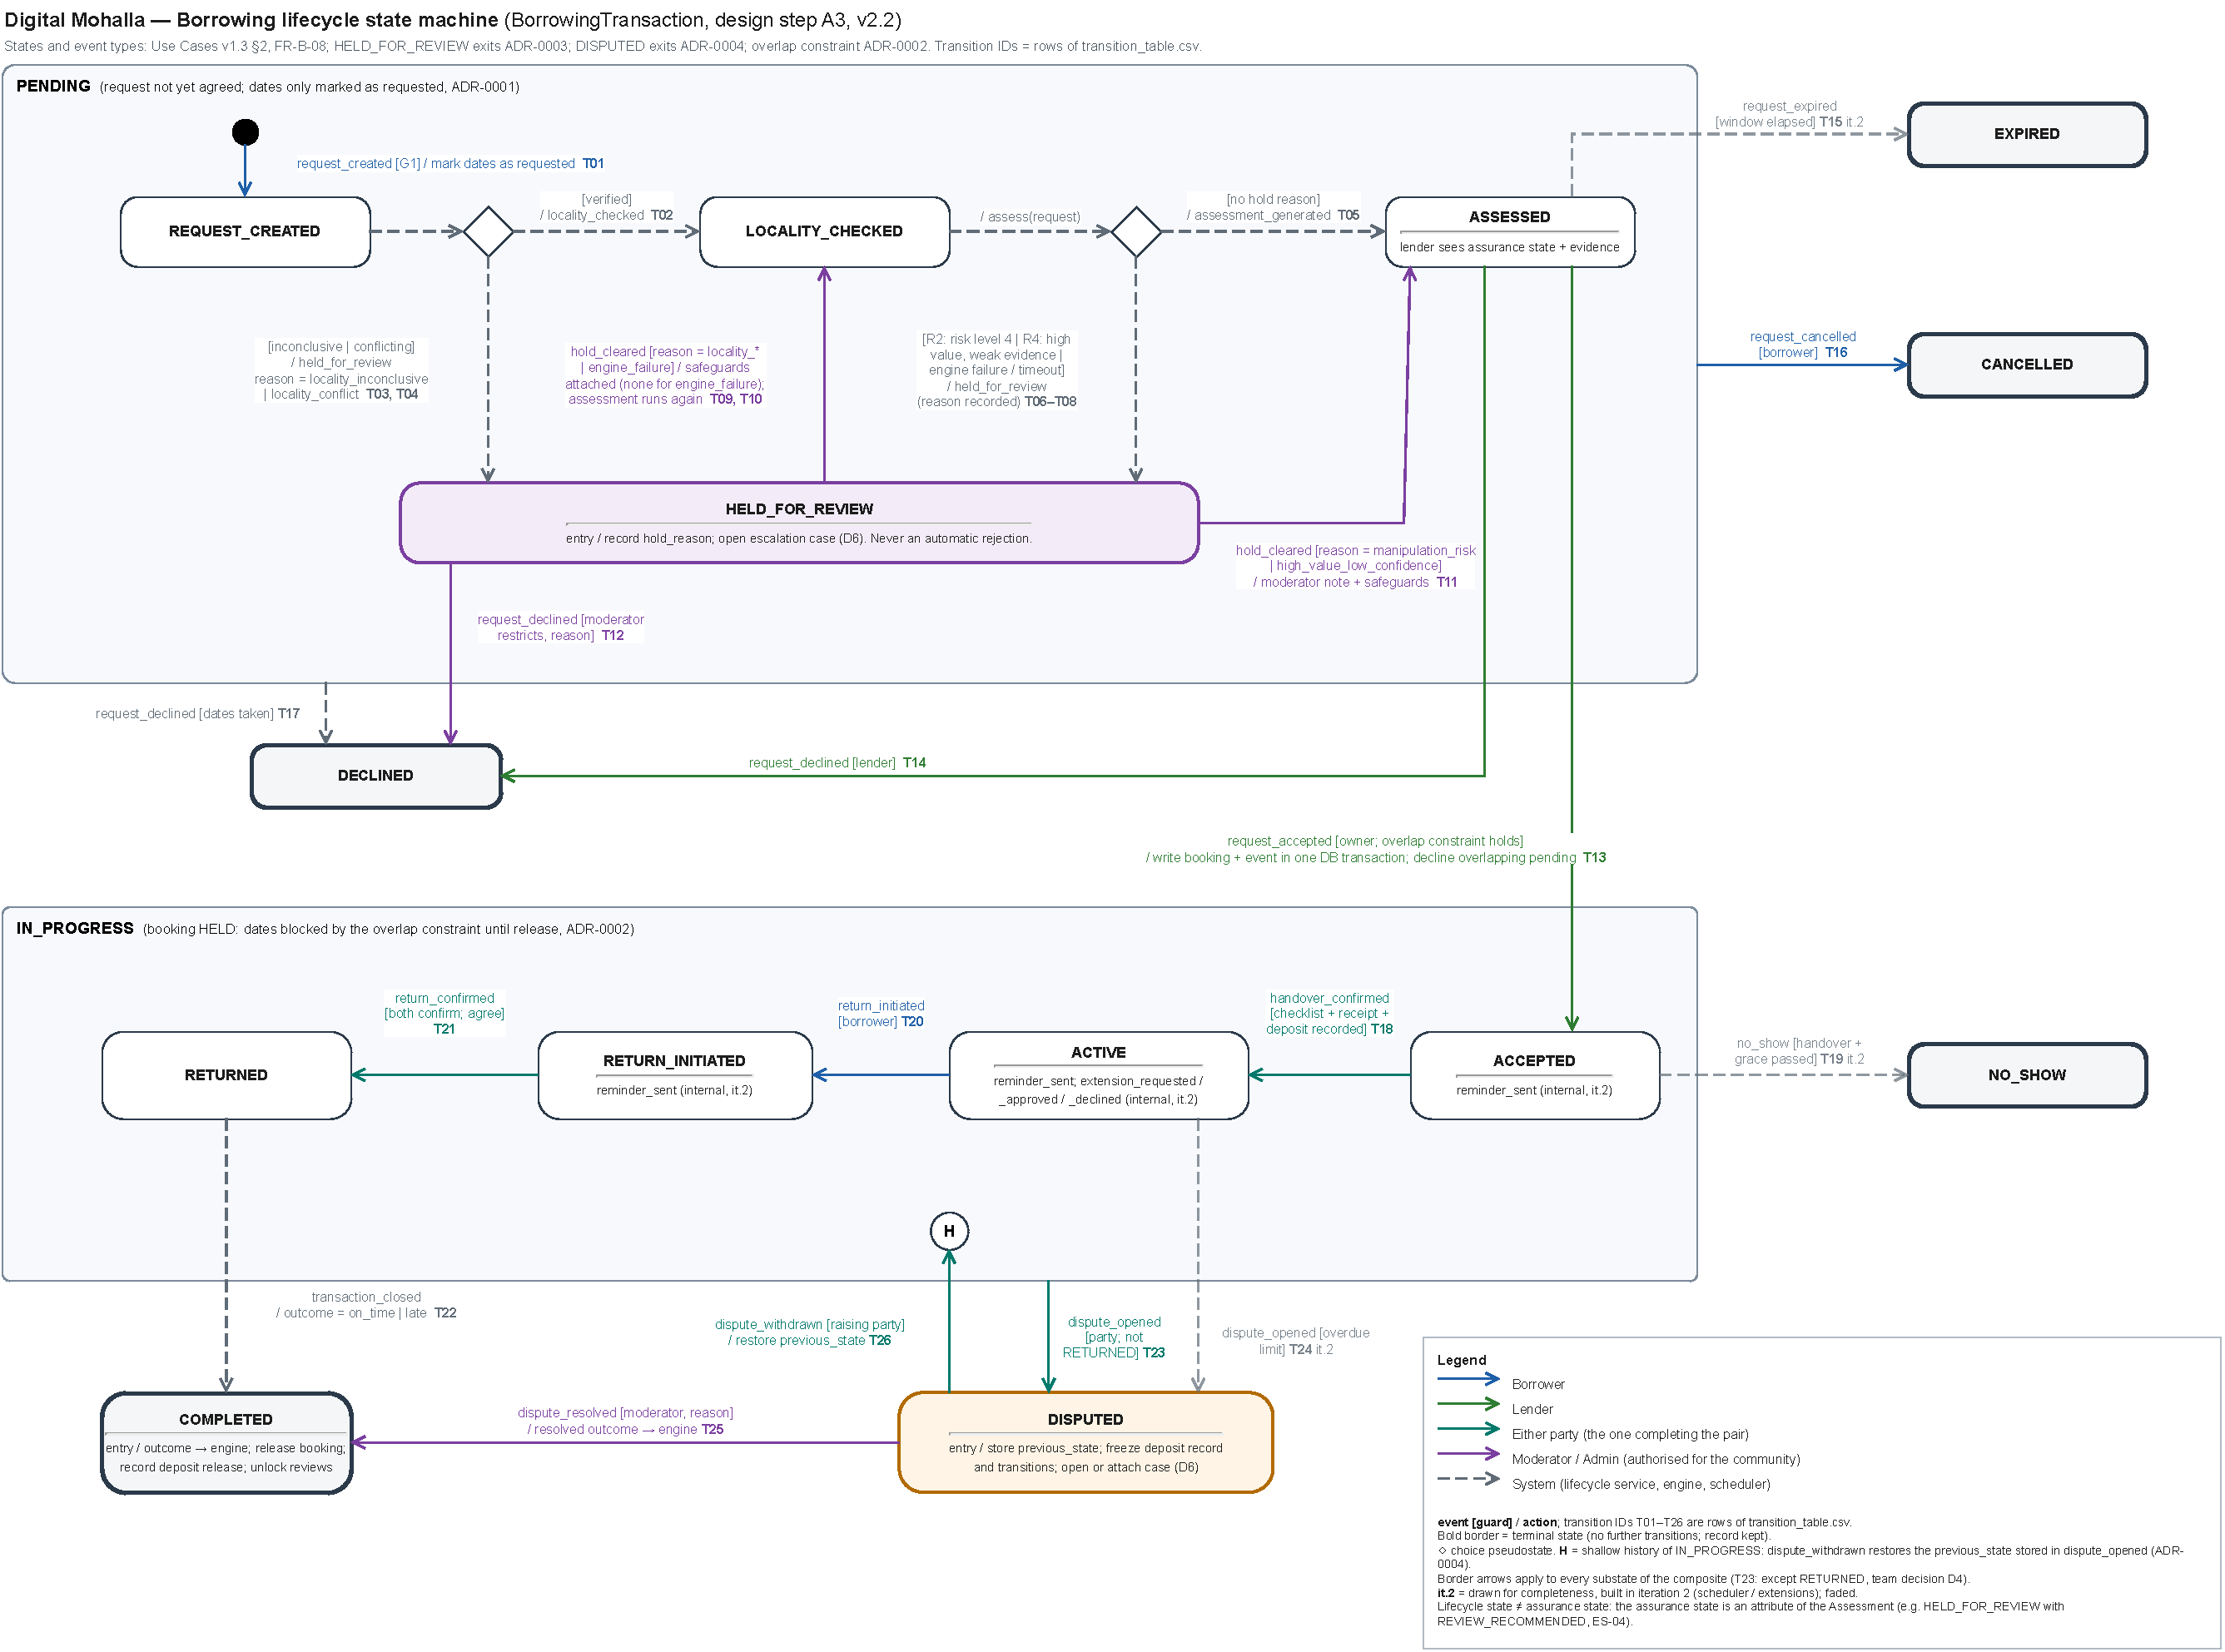
\includegraphics[width=\textwidth,height=0.80\textheight,keepaspectratio]{figures/diagrams/borrowing_lifecycle_state_machine}
\caption{Borrowing lifecycle state machine v2.2 (UML 2.5, design step A3)}\label{fig:borrowing-lifecycle-state-machine}
\drawionote{borrowing_lifecycle_state_machine}{docs/design/07_state_machines/borrowing_lifecycle_state_machine.drawio}
\end{minipage}
\end{figure}

\subsection{Escalation case}\label{sec:escalation-case}
\begin{figure}[htbp]
\centering
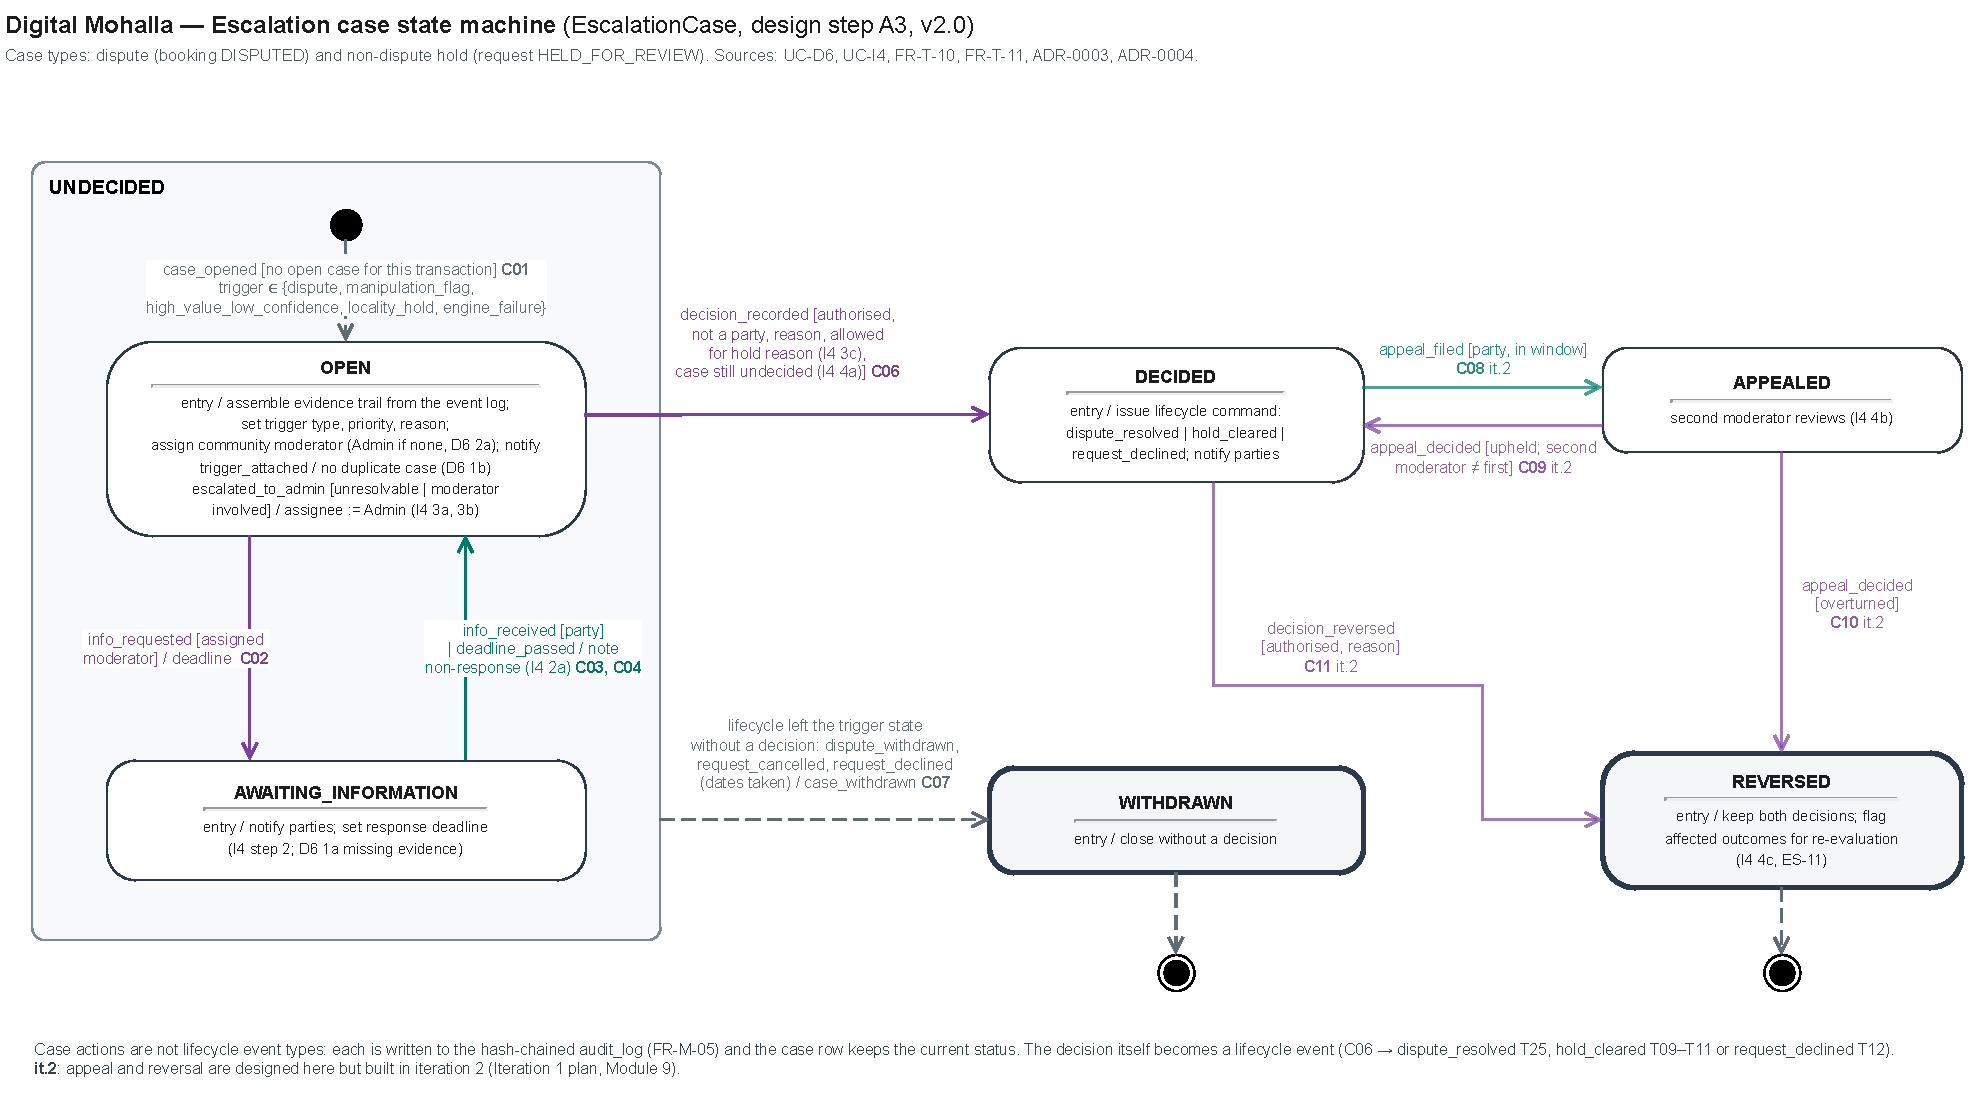
\includegraphics[width=\textwidth,height=0.80\textheight,keepaspectratio]{figures/diagrams/escalation_case_state_machine}
\caption{Escalation case state machine (UML 2.5, design step A3)}\label{fig:escalation-case-state-machine}
\drawionote{escalation_case_state_machine}{docs/design/07_state_machines/escalation_case_state_machine.drawio}
\end{figure}

\textbf{Reasoning.} A case opens for a dispute or a hold and ends either decided (with a mandatory reason) or withdrawn without a decision when the loan leaves the hold or dispute, for instance when the borrower cancels or withdraws (D9). A second dispute or hold on the same loan attaches to the open case instead of creating another (FR-T-10). A decision is stored append-only in \code{moderator_decision} and then applied as a lifecycle event in the hash-chained event log. Iteration 1 builds opening (C01), deciding (C06) and withdrawal (C07); information requests (C02--C04) and the appeal and reversal path (C08--C11) are built in Iteration 2. \textit{Serves:} FR-T-10, FR-T-11.

\subsection{Interactions}\label{sec:interactions}
\textbf{Reasoning.} The dispute freezes the loan and opens a case in the same database transaction as the \code{dispute_opened} event, so there is never a disputed loan without a case. The moderator's decision is first recorded (\code{moderator_decision}) and then applied as one lifecycle event that references it (\code{evidence_refs.decision_id}), so the decision and its effect cannot diverge. Sequence (b), handover to evidence, is in Appendix~\ref{app:additional-design-diagrams}. \textit{Serves:} FR-B-16, FR-T-10, FR-T-11. \textit{Owner:} S3.

\begin{figure}[p]
\centering
\begin{minipage}[c][0.92\textheight][c]{\textwidth}\centering
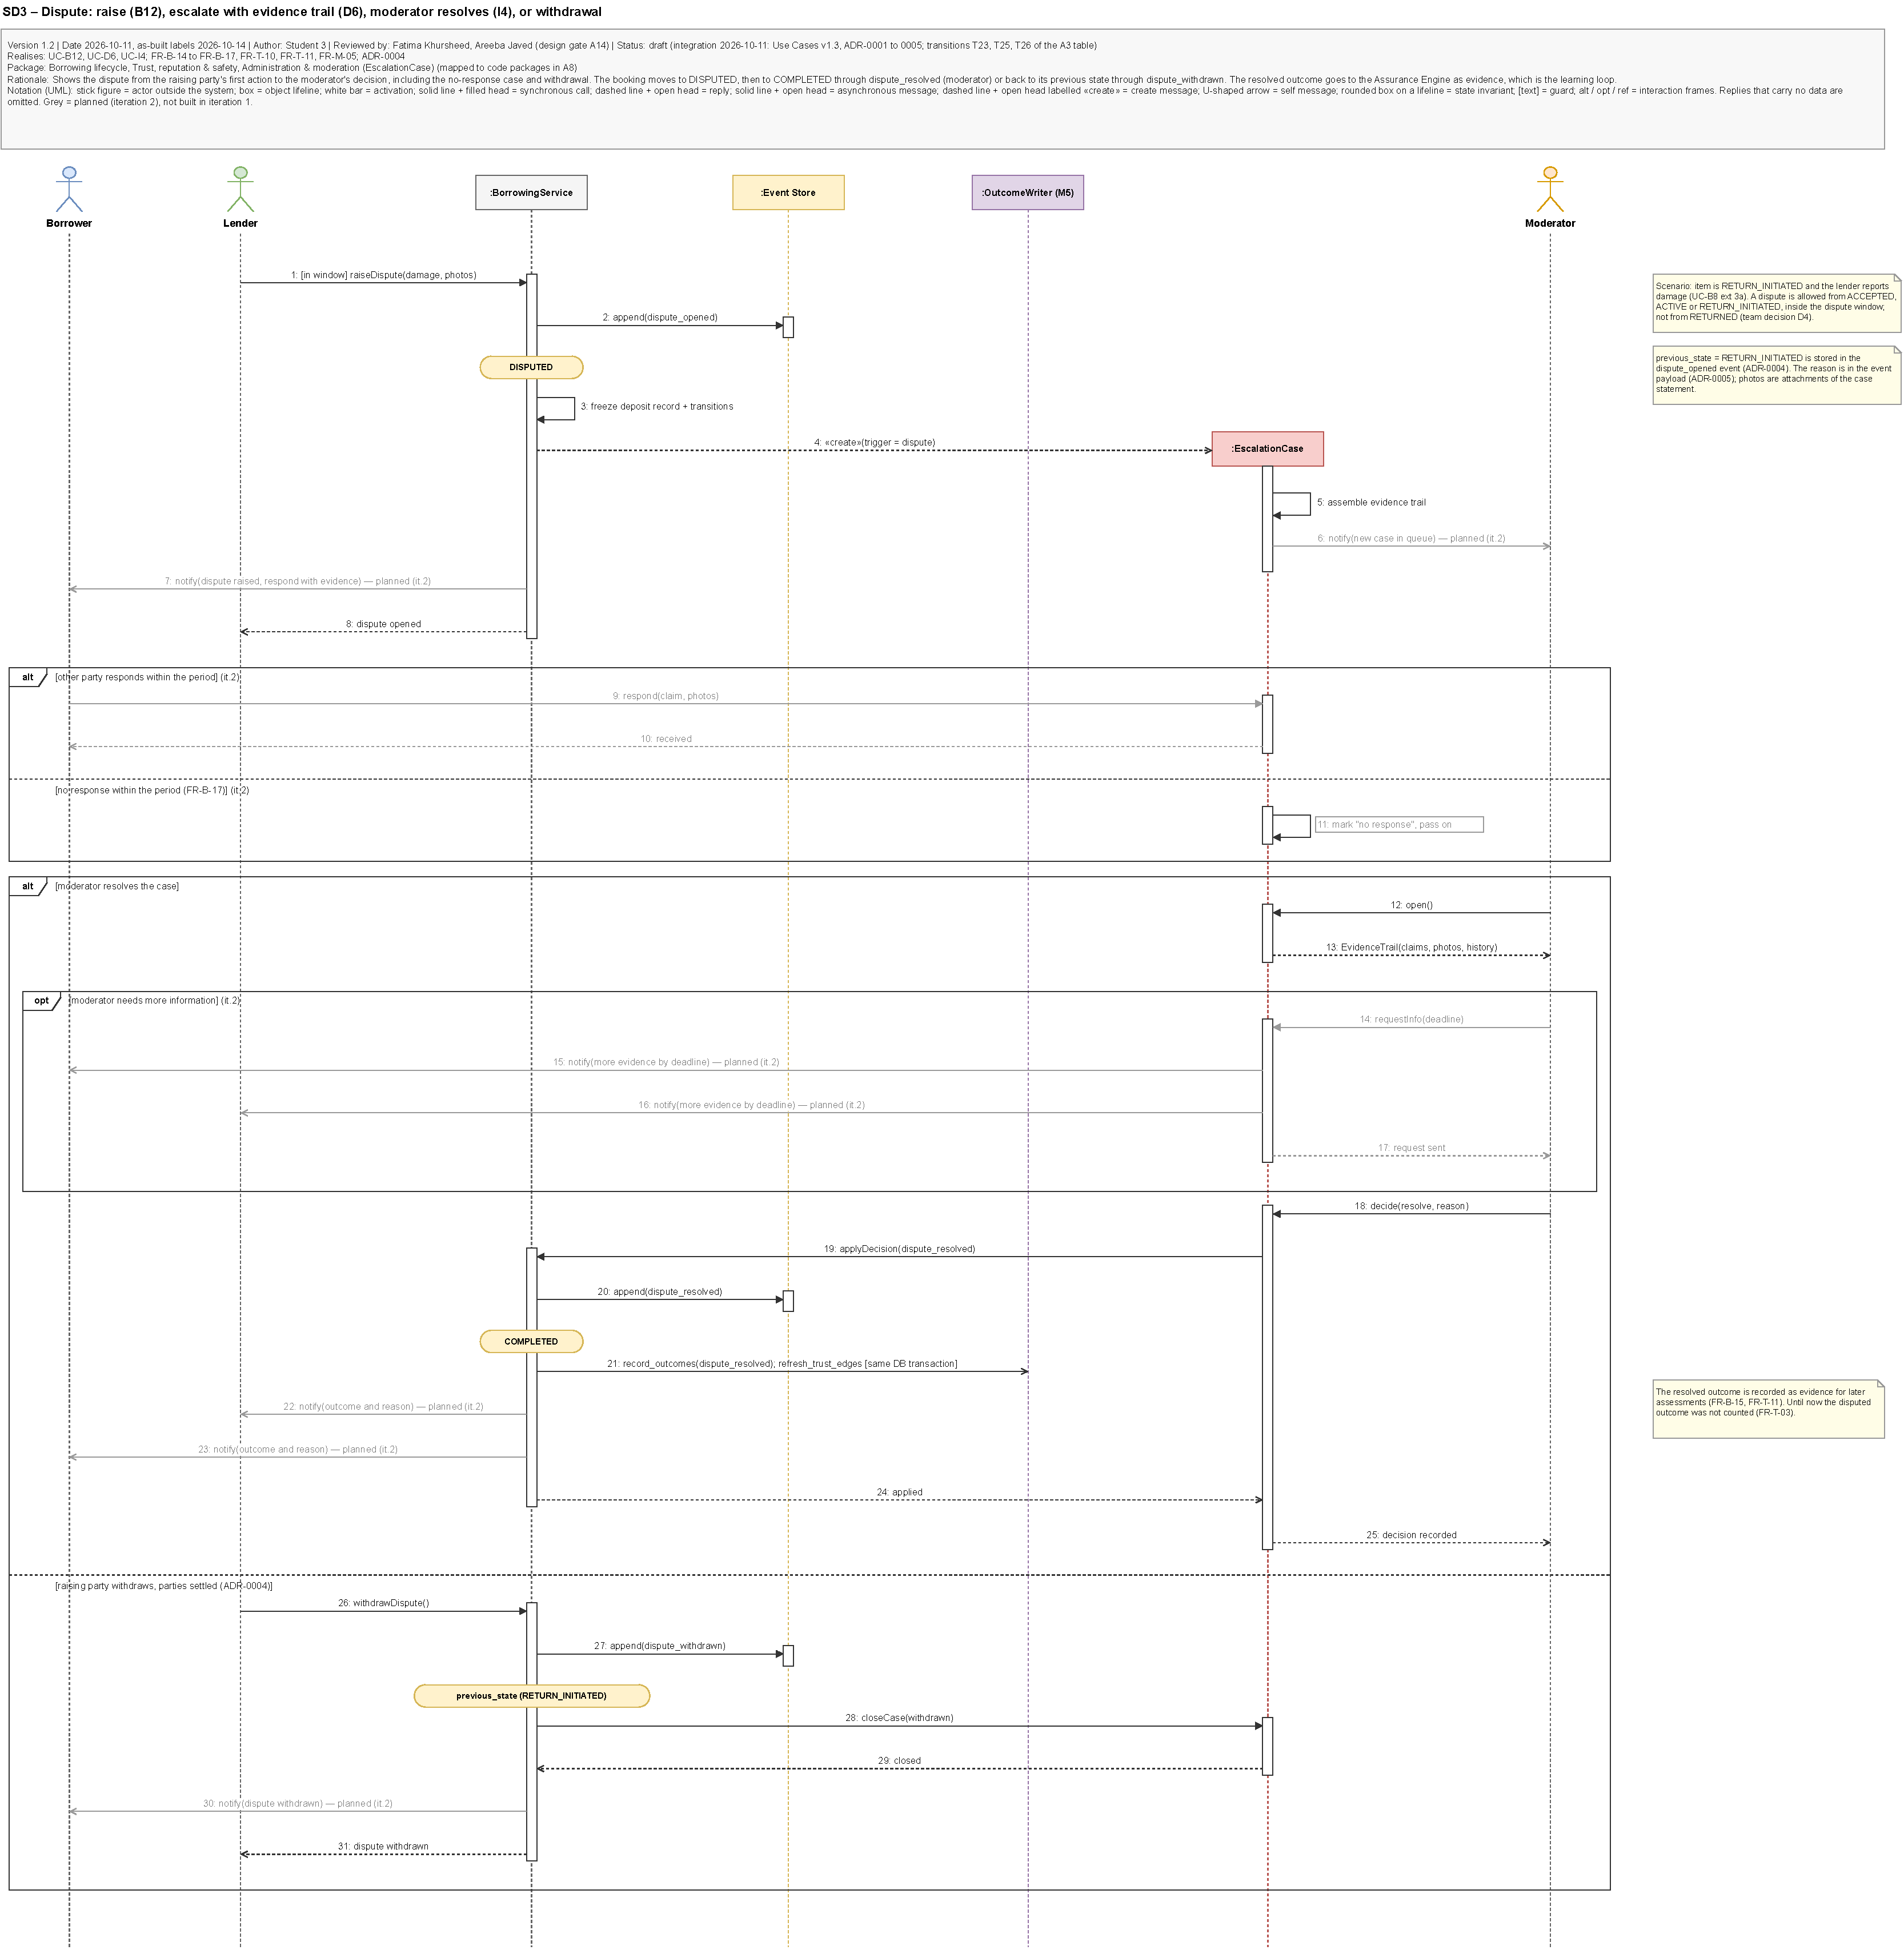
\includegraphics[width=\textwidth,height=0.80\textheight,keepaspectratio]{figures/diagrams/sequence_c_dispute}
\caption{Sequence (c): raise dispute, escalate, moderator decision (UC-B12, D6, I4)}\label{fig:sequence-c-dispute}
\drawionote{sequence_c_dispute}{docs/design/08_sequence_diagrams/sequence_c_dispute.drawio}
\end{minipage}
\end{figure}

\subsection{Data flow and privacy boundary}\label{sec:data-flow-privacy-boundary}
\begin{figure}[htbp]
\centering
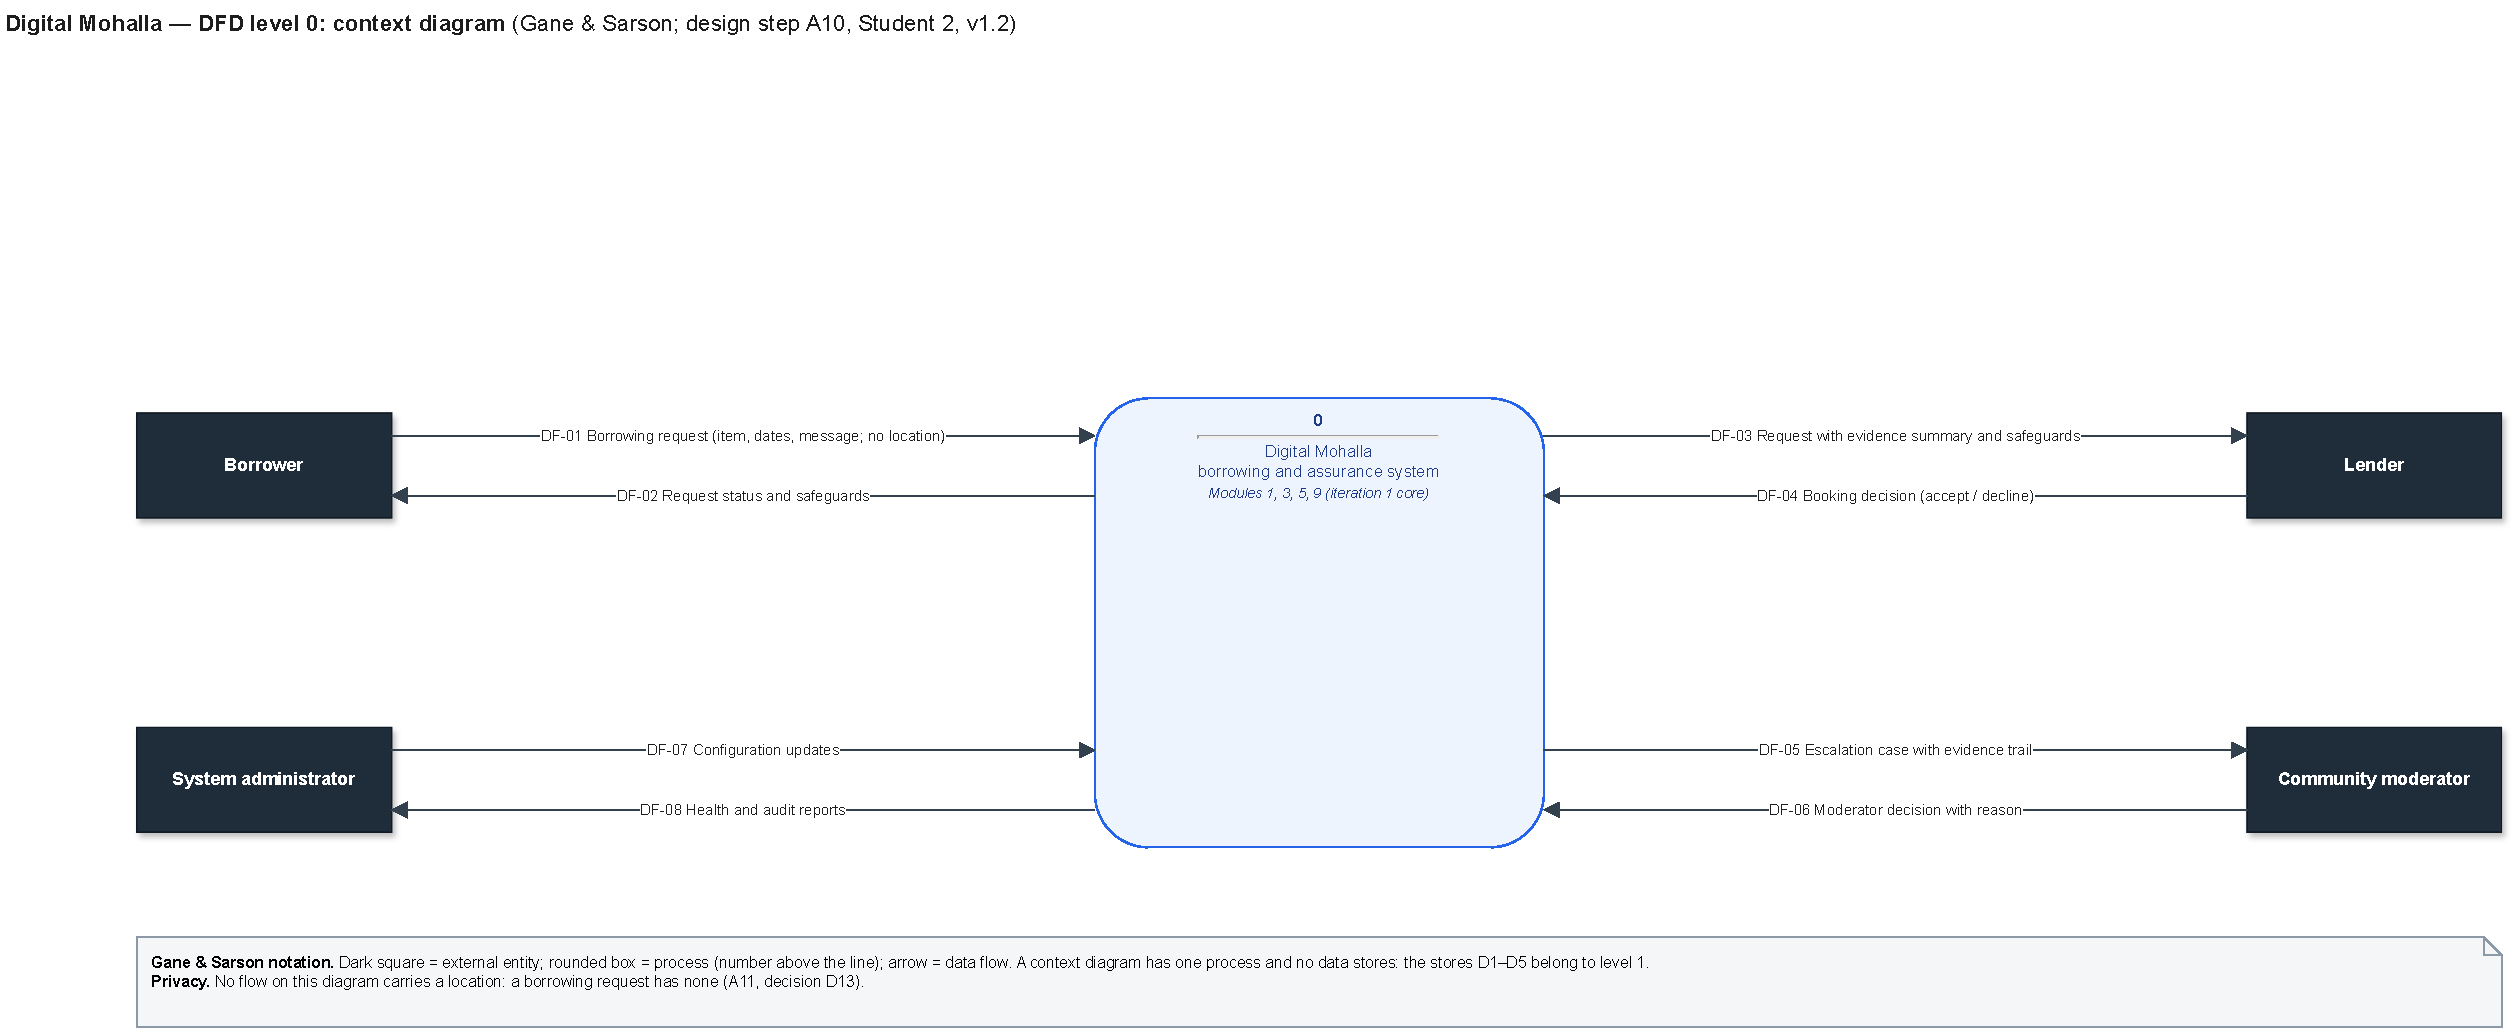
\includegraphics[width=\textwidth,height=0.80\textheight,keepaspectratio]{figures/diagrams/dfd_level0}
\caption{Assurance pipeline, DFD level 0 (context diagram; Gane and Sarson, design step A10)}\label{fig:dfd-level-0}
\drawionote{dfd_level0}{docs/design/10_dfd/dfd_assurance_pipeline_level0_level1.drawio}
\end{figure}

\textbf{Reasoning.} The context diagram shows what enters and leaves the assurance pipeline: lifecycle events and reviews in; assessments, explanations and cases out. Exact location never crosses into the pipeline: GPS is read only at membership time and reduced to a coarse result, and the request carries no location (D13). \textit{Serves:} NFR-PR-01, NFR-PR-02. \textit{Owner:} S2.

\subsection{Deployment}\label{sec:deployment}
\textbf{Reasoning and as-built deployment.} Figure~\ref{fig:deployment-diagram} shows the deployment as built; the provisional Part A design (one AWS host) is kept in Appendix~\ref{app:additional-design-diagrams} (Figure~\ref{fig:deployment-diagram-part-a}). The Part A design fixed what any target must provide: TLS termination, one API process, PostgreSQL 16 with \code{btree_gist}, migrations before start-up, a \code{/health} check and secrets outside the repository; it marked the host itself ``to be confirmed''. The confirmed target keeps every one of these properties on managed services. The API runs as a Docker container on Render (\code{digitalmohalla-api}) that applies \code{alembic upgrade head} and then starts Uvicorn; the web app is an Expo web export served by Render as a static site (\code{digitalmohalla-web}); the database is Neon PostgreSQL 16. Render deploys \code{main} only after the CI checks pass, and secrets live in Render's environment settings. \textit{Serves:} NFR-D-03, NFR-D-04, NFR-S-01.

\begin{figure}[htbp]
\centering
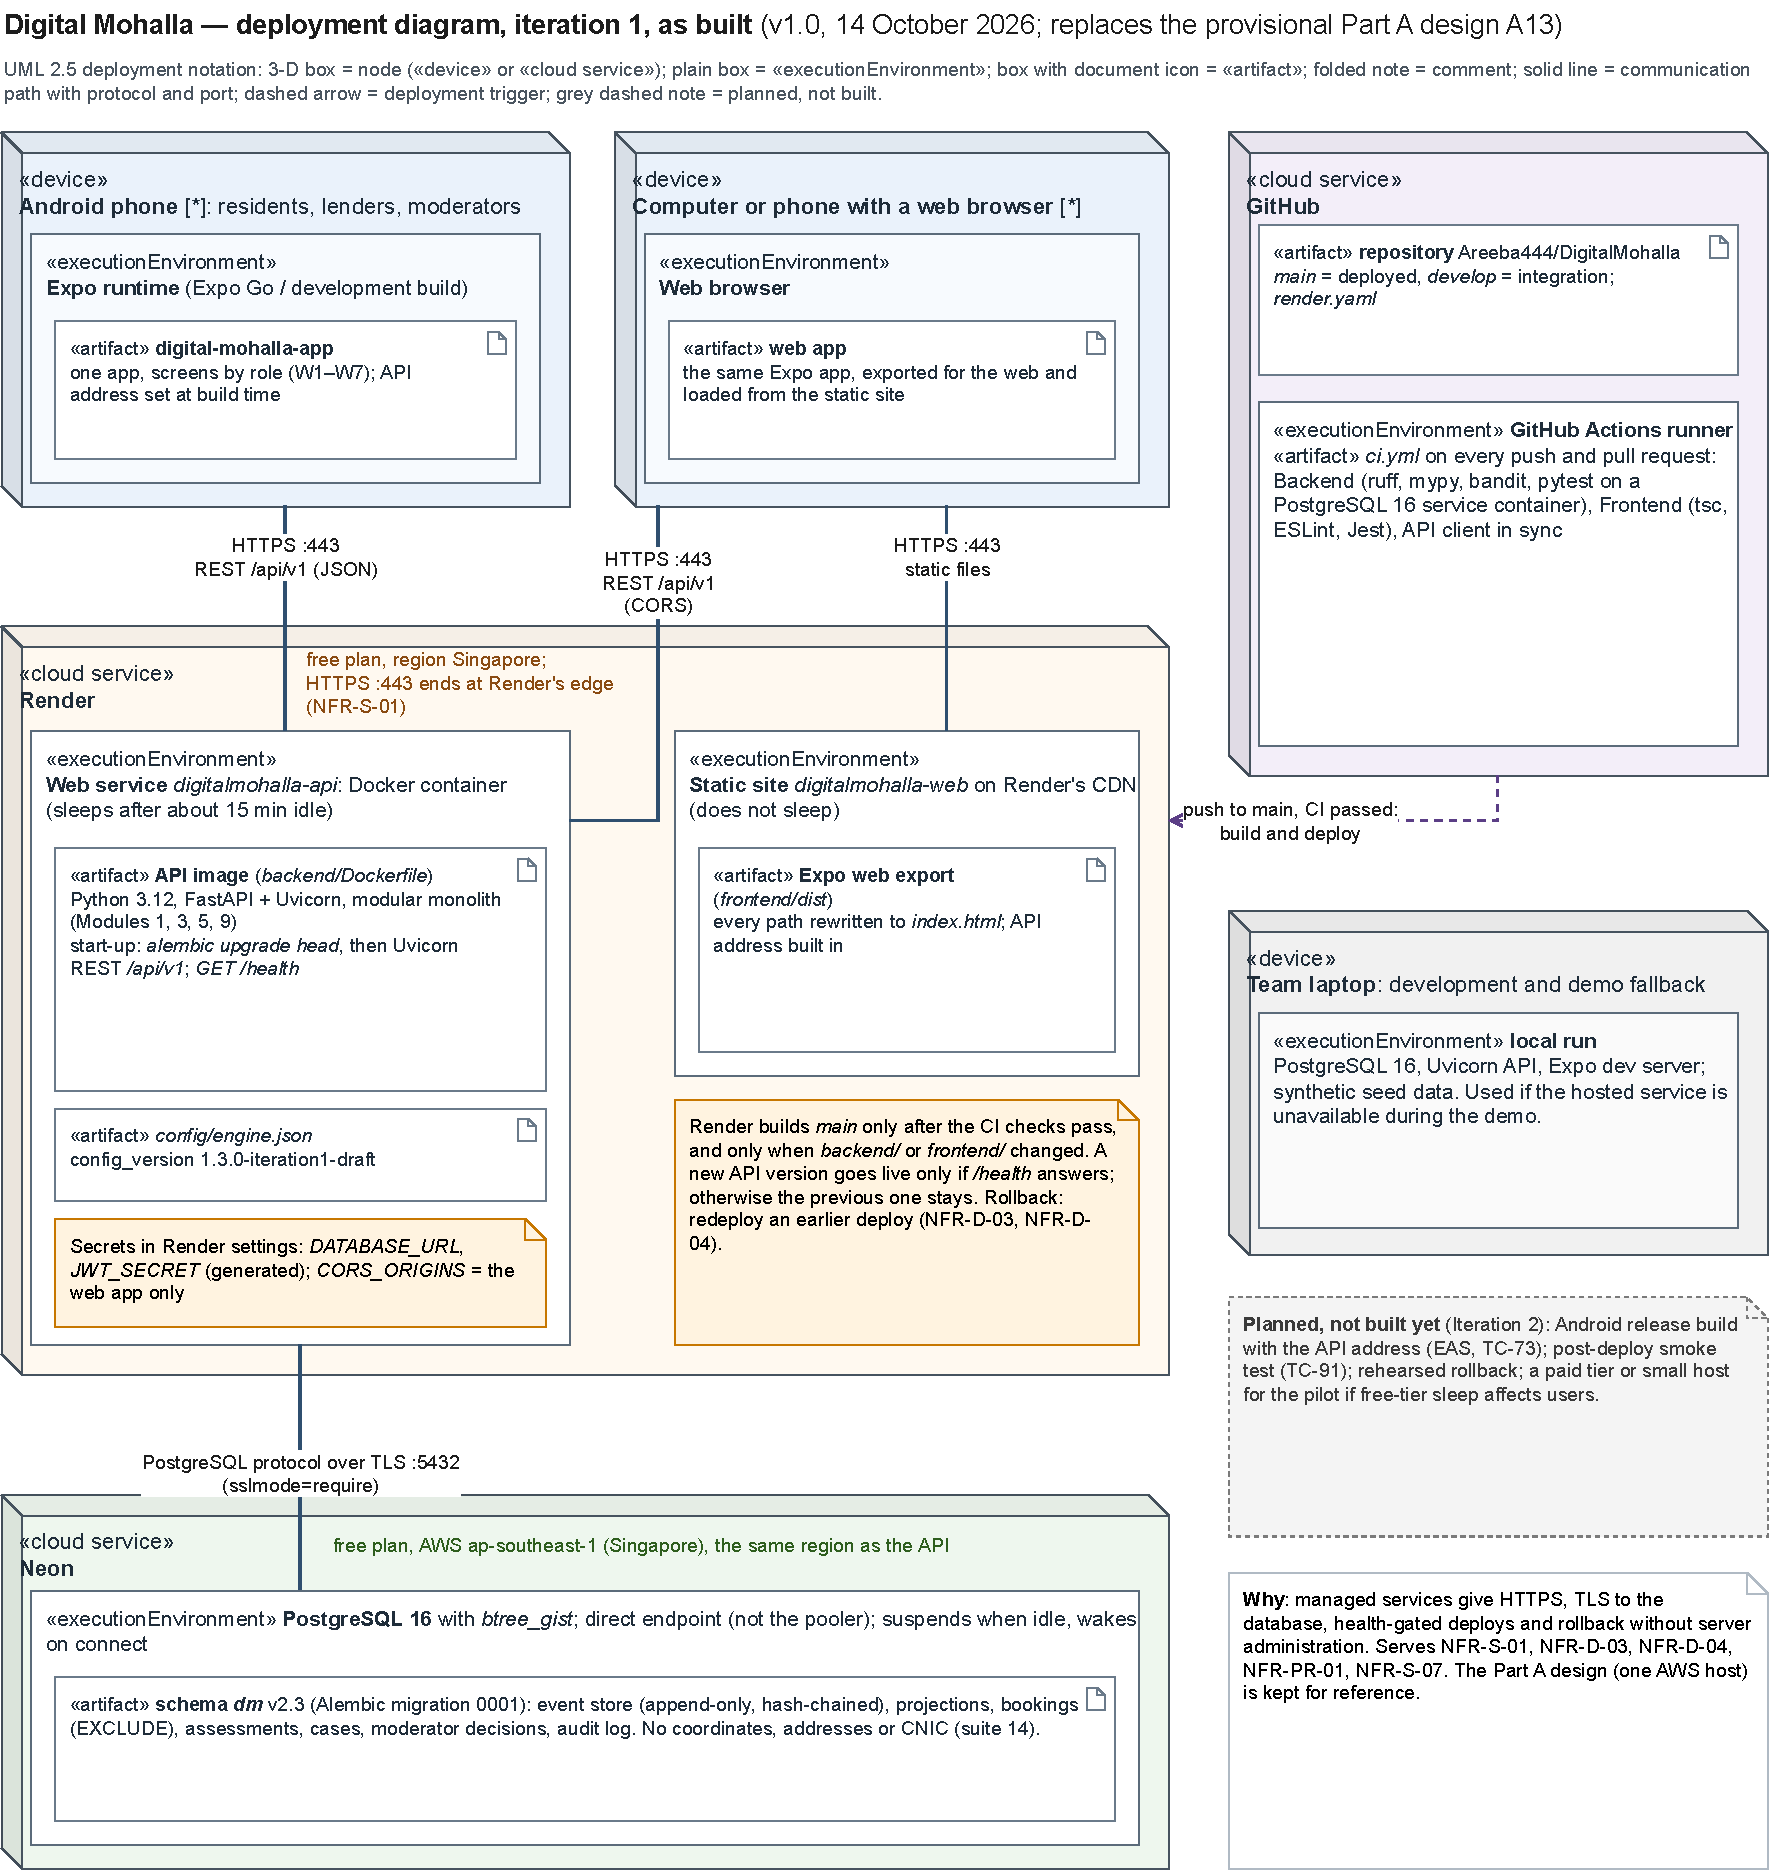
\includegraphics[width=\textwidth,height=0.80\textheight,keepaspectratio]{figures/diagrams/deployment_diagram}
\caption{Deployment diagram, Iteration 1 as built (UML 2.5): API and web app on Render, PostgreSQL 16 on Neon, deployed from \texttt{main} after CI passes}\label{fig:deployment-diagram}
\drawionote{deployment_diagram}{docs/design/04_deployment/deployment_diagram.drawio}
\end{figure}
